\documentclass[../../../main.tex]{subfiles}
\begin{document}

In the previous section, it was demonstrated that the viability of a solution cannot depend entirely on chance.
The use of uniform random point generation was ruled out in favour of Poisson-disk distribution because it was found that randomness had to be conditioned to make it viable. 
Even so, there is still too much variability in all aspects. 

In addition, the importance of the distribution of node connections was noted, and it was concluded that ensuring the continuity of the graph structure is not sufficient for the solution to be viable. 
Node connections can be classified as upper and lower depending on whether the connection is made with a point above or below it.
If a node only has one or two connections, above or below, it is not structurally stable. 
Each node should have at least four upper and lower connections to restrict its displacement when faced with the maximum possible load. 
Furthermore, ideally, these connections should be distributed around the node. It is useless if a node has many connections, but they all have the same orientation.
Finally, it was observed that controlling the length of the connections is also necessary to avoid intersections between edges.

In this subsection, a method derived from the previous one is proposed. 
The previous approach relied on full randomness to place the points and, as a result, many of the points were not placed in the correct locations and became isolated or lost continuity.
This method focuses on controlling the randomness to ensure that the randomly generated points end up in a more optimal location. 
To do this, a smaller number of points are generated in the volume, which, together with the points on the surface of the volume, will serve as seeds. 
From these seeds, it will be evaluated whether there are nearby points to join and if not, new points will be generated around these seeds at optimal locations.
In this way, the points are generated randomly but are modified to be valid, so this method has been considered pseudo-random.


\subsection{Random points generation on a spherical cap}\label{sec:random_gen}

It was noted that the position in which the nodes are generated is crucial to ensure the continuity of the system. 
Many points fall in locations where they form less than 45$^\circ$ with the evaluated node and are therefore invalid. Therefore, this methodology proposes to be able to modify these nodes to positions that are valid and can generate connections. 
If there are no points to modify, they can be generated during execution.
Those points generated during the execution would lie within an area that has been called the solution space. 
As done in the previous section, the connections of each node will be generated only upwards to avoid redundancies. 
The connections below a node are assured since the connections are reciprocal: if a node, $n_1$, is connected to another, $n_2$, above it, node $n_2$ is assured of a connection below with node $n_1$. 
Also, in the previous section, it was seen that it is important to keep connections as short as possible to avoid intersections. 
Therefore, the points generated from a node will be at a constant and common distance \textit{d} from that node. 
Thus, the solution space will be shaped like a hemisphere. 
However, within this solution space, only those that form a 45$^{\circ}$ angle will be valid, so instead of a hemispherical shape, the solution space will be shaped like a spherical cap as shown in \cref{fig:space_solution}.

\begin{figure}[!htbp]
    \centering
    

% Gradient Info
  
\tikzset {_e292ujfi3/.code = {\pgfsetadditionalshadetransform{ \pgftransformshift{\pgfpoint{513 bp } { -174 bp }  }  \pgftransformscale{3 }  }}}
\pgfdeclareradialshading{_n7edsi42z}{\pgfpoint{-176bp}{64bp}}{rgb(0bp)=(1,1,1);
rgb(0bp)=(1,1,1);
rgb(12.767857142857142bp)=(0.91,0.25,0.25);
rgb(400bp)=(0.91,0.25,0.25)}
\tikzset{every picture/.style={line width=0.75pt}} %set default line width to 0.75pt        

\begin{tikzpicture}[x=0.75pt,y=0.75pt,yscale=-1,xscale=1]
%uncomment if require: \path (0,300); %set diagram left start at 0, and has height of 300

%Shape: Chord [id:dp241657055871786] 
\draw   (193.93,190.4) .. controls (194.07,136.1) and (244.83,92.15) .. (307.4,92.19) .. controls (369.93,92.23) and (420.61,136.21) .. (420.74,190.46) -- cycle ;
%Curve Lines [id:da7774614939439684] 
\draw [shading=_n7edsi42z,_e292ujfi3]   (232.9,116.25) .. controls (253.33,99.17) and (321.67,70.17) .. (382.5,117.25) ;
%Shape: Boxed Bezier Curve [id:dp976459988898636] 
\draw [fill={rgb, 255:red, 232; green, 63; blue, 63 }  ,fill opacity=1 ]   (232.5,116) .. controls (246.19,123.48) and (280.95,126.81) .. (314,126.48) .. controls (325.54,126.36) and (336.87,125.79) .. (347.02,124.8) .. controls (363.03,123.24) and (376.13,120.61) .. (382.5,117) ;
%Shape: Circle [id:dp060964936174491724] 
\draw  [fill={rgb, 255:red, 0; green, 0; blue, 0 }  ,fill opacity=1 ] (307.13,190.4) .. controls (307.13,188.54) and (308.64,187.03) .. (310.51,187.03) .. controls (312.37,187.03) and (313.88,188.54) .. (313.88,190.4) .. controls (313.88,192.27) and (312.37,193.78) .. (310.51,193.78) .. controls (308.64,193.78) and (307.13,192.27) .. (307.13,190.4) -- cycle ;
%Straight Lines [id:da1793972926995161] 
\draw    (232.9,116.25) -- (247.22,129.93) -- (310.51,190.4) ;
%Straight Lines [id:da6269963502636927] 
\draw    (380.39,119.38) -- (308.38,192.13) ;
\draw [shift={(382.5,117.25)}, rotate = 134.71] [fill={rgb, 255:red, 0; green, 0; blue, 0 }  ][line width=0.08]  [draw opacity=0] (6.25,-3) -- (0,0) -- (6.25,3) -- cycle    ;
%Straight Lines [id:da5790726192958345] 
\draw    (310.51,190.4) -- (353.08,190.39) ;
\draw [shift={(356.08,190.39)}, rotate = 179.98] [fill={rgb, 255:red, 0; green, 0; blue, 0 }  ][line width=0.08]  [draw opacity=0] (3.57,-1.72) -- (0,0) -- (3.57,1.72) -- cycle    ;
%Shape: Arc [id:dp6972628103446205] 
\draw  [draw opacity=0] (327.33,173.18) .. controls (329.4,175.4) and (331.16,177.98) .. (332.51,180.87) .. controls (334.05,184.13) and (334.94,187.53) .. (335.24,190.93) -- (305.36,193.62) -- cycle ; \draw    (329.27,175.5) .. controls (330.51,177.14) and (331.6,178.93) .. (332.51,180.87) .. controls (334.05,184.13) and (334.94,187.53) .. (335.24,190.93) ;  \draw [shift={(327.33,173.18)}, rotate = 47.09] [fill={rgb, 255:red, 0; green, 0; blue, 0 }  ][line width=0.08]  [draw opacity=0] (3.57,-1.72) -- (0,0) -- (3.57,1.72) -- cycle    ;
%Straight Lines [id:da5528525747103438] 
\draw    (310.21,44.4) -- (310.51,190.4) ;
\draw [shift={(310.2,41.4)}, rotate = 89.88] [fill={rgb, 255:red, 0; green, 0; blue, 0 }  ][line width=0.08]  [draw opacity=0] (3.57,-1.72) -- (0,0) -- (3.57,1.72) -- cycle    ;
%Straight Lines [id:da8340088843622058] 
\draw    (292.37,207.73) -- (310.51,190.4) ;
\draw [shift={(290.2,209.8)}, rotate = 316.31] [fill={rgb, 255:red, 0; green, 0; blue, 0 }  ][line width=0.08]  [draw opacity=0] (3.57,-1.72) -- (0,0) -- (3.57,1.72) -- cycle    ;
%Curve Lines [id:da6149455400699015] 
\draw  [dash pattern={on 0.84pt off 2.51pt}]  (232.9,116.25) .. controls (277.35,100.09) and (376.33,112.17) .. (382.5,117.25) ;
%Shape: Pie [id:dp4766908428725254] 
\draw   (420.72,190.14) .. controls (420.73,190.25) and (420.74,190.36) .. (420.74,190.46) .. controls (420.74,201.51) and (369.96,210.46) .. (307.33,210.46) .. controls (244.78,210.46) and (194.05,201.53) .. (193.93,190.5) -- (307.33,190.46) -- cycle ;
%Shape: Arc [id:dp28428573759108733] 
\draw  [draw opacity=0][dash pattern={on 0.84pt off 2.51pt}] (193.97,190.87) .. controls (193.94,190.69) and (193.93,190.51) .. (193.93,190.34) .. controls (193.93,179.29) and (244.7,170.34) .. (307.33,170.34) .. controls (366.46,170.34) and (415.02,178.32) .. (420.27,188.5) -- (307.33,190.34) -- cycle ; \draw  [dash pattern={on 0.84pt off 2.51pt}] (193.97,190.87) .. controls (193.94,190.69) and (193.93,190.51) .. (193.93,190.34) .. controls (193.93,179.29) and (244.7,170.34) .. (307.33,170.34) .. controls (366.46,170.34) and (415.02,178.32) .. (420.27,188.5) ;  
%Shape: Arc [id:dp41874576724679013] 
\draw  [draw opacity=0] (298.58,201.75) .. controls (292.94,201.07) and (287.32,199.03) .. (282.43,195.59) .. controls (280.23,194.04) and (278.32,192.3) .. (276.71,190.44) -- (299.99,176.96) -- cycle ; \draw    (298.58,201.75) .. controls (292.94,201.07) and (287.32,199.03) .. (282.43,195.59) .. controls (281.1,194.65) and (279.88,193.65) .. (278.76,192.58) ; \draw [shift={(276.71,190.44)}, rotate = 47.4] [fill={rgb, 255:red, 0; green, 0; blue, 0 }  ][line width=0.08]  [draw opacity=0] (3.57,-1.72) -- (0,0) -- (3.57,1.72) -- cycle    ; 

% Text Node
\draw (338.16,141.1) node [anchor=north west][inner sep=0.75pt]  [font=\scriptsize] [align=left] {$\displaystyle d$};
% Text Node
\draw (312.51,193) node [anchor=north west][inner sep=0.75pt]  [font=\scriptsize] [align=left] {$\displaystyle n$};
% Text Node
\draw (300,202) node [anchor=north west][inner sep=0.75pt]  [font=\scriptsize] [align=left] {$\displaystyle x$};
% Text Node
\draw (342.37,192) node [anchor=north west][inner sep=0.75pt]  [font=\scriptsize] [align=left] {$\displaystyle y$};
% Text Node
\draw (313.59,42.6) node [anchor=north west][inner sep=0.75pt]  [font=\scriptsize] [align=left] {$\displaystyle z$};
% Text Node
\draw (336.4,172.8) node [anchor=north west][inner sep=0.75pt]  [font=\scriptsize] [align=left] {$\displaystyle \varphi =\ 45^{\circ }$};
% Text Node
\draw (272.8,195.4) node [anchor=north west][inner sep=0.75pt]  [font=\scriptsize] [align=left] {$\displaystyle \theta $};


\end{tikzpicture}

    \caption{Illustration of the solution space for node \textit{n}. The area of valid solutions is shown in red.}
    \label{fig:space_solution}
\end{figure}

However, instead of generating four random points in the solution space, it is proposed to divide the solution space into four quadrants and generate a random point in each quadrant.
This ensures that the connections of each node are distributed around it, providing greater stability to the node. This ensures that each node has at least four connections above it. 
This ensures that the connections of each node are distributed around it, providing greater stability to the node.
Quadrants are defined as a Cartesian coordinate system projected onto the solution space, and their designation follows the same criteria as the Cartesian system, \cref{fig:quadrants}. 
To find out which quadrant a point belongs to, the vector connecting that point to the node is obtained, and depending on the sign of its \textit{x} and \textit{y} coordinates, it will be classified in a quadrant.

\begin{figure}[!htbp]
    \centering
    

\tikzset{every picture/.style={line width=0.75pt}} %set default line width to 0.75pt        

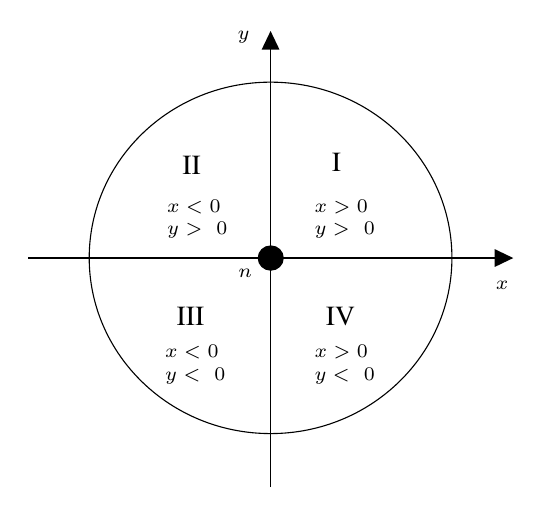
\begin{tikzpicture}[x=0.75pt,y=0.75pt,yscale=-1,xscale=1]
%uncomment if require: \path (0,300); %set diagram left start at 0, and has height of 300

%Shape: Ellipse [id:dp6073267521119902] 
\draw   (144.38,119.54) .. controls (144.38,72.78) and (183.5,34.88) .. (231.76,34.88) .. controls (280.01,34.88) and (319.13,72.78) .. (319.13,119.54) .. controls (319.13,166.29) and (280.01,204.2) .. (231.76,204.2) .. controls (183.5,204.2) and (144.38,166.29) .. (144.38,119.54) -- cycle ;
%Straight Lines [id:da17835254540908585] 
\draw    (115,119.62) -- (345.69,119.62) ;
\draw [shift={(348.69,119.62)}, rotate = 180] [fill={rgb, 255:red, 0; green, 0; blue, 0 }  ][line width=0.08]  [draw opacity=0] (8.93,-4.29) -- (0,0) -- (8.93,4.29) -- cycle    ;
%Straight Lines [id:da3214817137263065] 
\draw    (231.76,230) -- (231.76,13.24) ;
\draw [shift={(231.76,10.24)}, rotate = 90] [fill={rgb, 255:red, 0; green, 0; blue, 0 }  ][line width=0.08]  [draw opacity=0] (8.93,-4.29) -- (0,0) -- (8.93,4.29) -- cycle    ;
%Shape: Ellipse [id:dp010903733793728554] 
\draw  [fill={rgb, 255:red, 0; green, 0; blue, 0 }  ,fill opacity=1 ] (225.83,119.62) .. controls (225.83,116.4) and (228.52,113.8) .. (231.84,113.8) .. controls (235.17,113.8) and (237.86,116.4) .. (237.86,119.62) .. controls (237.86,122.84) and (235.17,125.45) .. (231.84,125.45) .. controls (228.52,125.45) and (225.83,122.84) .. (225.83,119.62) -- cycle ;

% Text Node
\draw (260,67.69) node [anchor=north west][inner sep=0.75pt]   [align=left] {{\fontfamily{ptm}\selectfont I}};
% Text Node
\draw (188.04,69) node [anchor=north west][inner sep=0.75pt]   [align=left] {{\fontfamily{ptm}\selectfont II}};
% Text Node
\draw (185.23,142) node [anchor=north west][inner sep=0.75pt]   [align=left] {{\fontfamily{ptm}\selectfont III}};
% Text Node
\draw (257.15,142) node [anchor=north west][inner sep=0.75pt]   [align=left] {{\fontfamily{ptm}\selectfont IV}};
% Text Node
\draw (214.66,8.9) node [anchor=north west][inner sep=0.75pt]  [font=\scriptsize] [align=left] {$\displaystyle y$};
% Text Node
\draw (339.06,129.44) node [anchor=north west][inner sep=0.75pt]  [font=\scriptsize] [align=left] {$\displaystyle x$};
% Text Node
\draw (245,89) node [anchor=north west][inner sep=0.75pt]  [font=\scriptsize] [align=left] {$\displaystyle  \begin{array}{{>{\displaystyle}l}}
x >0\\
y >\ 0
\end{array}$};
% Text Node
\draw (174,89) node [anchor=north west][inner sep=0.75pt]  [font=\scriptsize] [align=left] {$\displaystyle  \begin{array}{{>{\displaystyle}l}}
x< 0\\
y >\ 0
\end{array}$};
% Text Node
\draw (173,159) node [anchor=north west][inner sep=0.75pt]  [font=\scriptsize] [align=left] {$\displaystyle  \begin{array}{{>{\displaystyle}l}}
x< 0\\
y< \ 0
\end{array}$};
% Text Node
\draw (245,159) node [anchor=north west][inner sep=0.75pt]  [font=\scriptsize] [align=left] {$\displaystyle  \begin{array}{{>{\displaystyle}l}}
x >0\\
y< \ 0
\end{array}$};
% Text Node
\draw (215,123.5) node [anchor=north west][inner sep=0.75pt]  [font=\scriptsize] [align=left] {$\displaystyle n$};


\end{tikzpicture}

    \caption{Definition of the four quadrants and the coordinate signs in each of them. }
    \label{fig:quadrants}
\end{figure}

\cref{fig:quadrants_ex} shows an example of how four points distributed in each of the quadrants would look from an isometric and floor plan.
This is the goal to be achieved. But to achieve it, it is first necessary to be able to generate random points within each of the quadrants. 
At this point, randomness can be used as a resource because the possible results have been narrowed down so much that any one of them will be valid. 

\begin{figure}[!htbp]
    \centering
    

% Gradient Info
  
\tikzset {_ectzm6pjz/.code = {\pgfsetadditionalshadetransform{ \pgftransformshift{\pgfpoint{9.5 bp } { 15.5 bp }  }  \pgftransformscale{1 }  }}}
\pgfdeclareradialshading{_ahugjddyw}{\pgfpoint{0bp}{0bp}}{rgb(0bp)=(1,1,1);
rgb(0bp)=(1,1,1);
rgb(25bp)=(0.82,0.01,0.11);
rgb(400bp)=(0.82,0.01,0.11)}

% Gradient Info
  
\tikzset {_th1cm3in6/.code = {\pgfsetadditionalshadetransform{ \pgftransformshift{\pgfpoint{9.5 bp } { 15.5 bp }  }  \pgftransformscale{1 }  }}}
\pgfdeclareradialshading{_d1dtwgk5f}{\pgfpoint{0bp}{0bp}}{rgb(0bp)=(1,1,1);
rgb(0bp)=(1,1,1);
rgb(25bp)=(0.97,0.91,0.11);
rgb(400bp)=(0.97,0.91,0.11)}

% Gradient Info
  
\tikzset {_zhr1fu2w4/.code = {\pgfsetadditionalshadetransform{ \pgftransformshift{\pgfpoint{9.5 bp } { 15.5 bp }  }  \pgftransformscale{1 }  }}}
\pgfdeclareradialshading{_1ut9eedgr}{\pgfpoint{0bp}{0bp}}{rgb(0bp)=(1,1,1);
rgb(0bp)=(1,1,1);
rgb(25bp)=(0.72,0.91,0.53);
rgb(400bp)=(0.72,0.91,0.53)}
\tikzset{_809g6ggoh/.code = {\pgfsetadditionalshadetransform{\pgftransformshift{\pgfpoint{9.5 bp } { 15.5 bp }  }  \pgftransformscale{1 } }}}
\pgfdeclareradialshading{_nd18wnqfs} { \pgfpoint{0bp} {0bp}} {color(0bp)=(transparent!0);
color(0bp)=(transparent!0);
color(25bp)=(transparent!50);
color(400bp)=(transparent!50)} 
\pgfdeclarefading{_5lgbtl41j}{\tikz \fill[shading=_nd18wnqfs,_809g6ggoh] (0,0) rectangle (50bp,50bp); } 

% Gradient Info
  
\tikzset {_0mv3s2zfu/.code = {\pgfsetadditionalshadetransform{ \pgftransformshift{\pgfpoint{9.5 bp } { 15.5 bp }  }  \pgftransformscale{1 }  }}}
\pgfdeclareradialshading{_byc674lfj}{\pgfpoint{0bp}{0bp}}{rgb(0bp)=(1,1,1);
rgb(0bp)=(1,1,1);
rgb(25bp)=(0.29,0.56,0.89);
rgb(400bp)=(0.29,0.56,0.89)}
\tikzset{_kgqqhn495/.code = {\pgfsetadditionalshadetransform{\pgftransformshift{\pgfpoint{9.5 bp } { 15.5 bp }  }  \pgftransformscale{1 } }}}
\pgfdeclareradialshading{_iqidbwe0j} { \pgfpoint{0bp} {0bp}} {color(0bp)=(transparent!0);
color(0bp)=(transparent!0);
color(25bp)=(transparent!50);
color(400bp)=(transparent!50)} 
\pgfdeclarefading{_zuztfk56c}{\tikz \fill[shading=_iqidbwe0j,_kgqqhn495] (0,0) rectangle (50bp,50bp); } 

% Gradient Info
  
\tikzset {_iddht9xy5/.code = {\pgfsetadditionalshadetransform{ \pgftransformshift{\pgfpoint{9.5 bp } { 15.5 bp }  }  \pgftransformscale{1 }  }}}
\pgfdeclareradialshading{_96md7qt0n}{\pgfpoint{0bp}{0bp}}{rgb(0bp)=(1,1,1);
rgb(0bp)=(1,1,1);
rgb(25bp)=(0.82,0.01,0.11);
rgb(400bp)=(0.82,0.01,0.11)}

% Gradient Info
  
\tikzset {_upwrgh5t1/.code = {\pgfsetadditionalshadetransform{ \pgftransformshift{\pgfpoint{9.5 bp } { 15.5 bp }  }  \pgftransformscale{1 }  }}}
\pgfdeclareradialshading{_1vnog2y7n}{\pgfpoint{0bp}{0bp}}{rgb(0bp)=(1,1,1);
rgb(0bp)=(1,1,1);
rgb(25bp)=(0.29,0.56,0.89);
rgb(400bp)=(0.29,0.56,0.89)}

% Gradient Info
  
\tikzset {_o60vc6flc/.code = {\pgfsetadditionalshadetransform{ \pgftransformshift{\pgfpoint{9.5 bp } { 15.5 bp }  }  \pgftransformscale{1 }  }}}
\pgfdeclareradialshading{_7owy0tp3f}{\pgfpoint{0bp}{0bp}}{rgb(0bp)=(1,1,1);
rgb(0bp)=(1,1,1);
rgb(25bp)=(0.97,0.91,0.11);
rgb(400bp)=(0.97,0.91,0.11)}

% Gradient Info
  
\tikzset {_u7bjhmdgn/.code = {\pgfsetadditionalshadetransform{ \pgftransformshift{\pgfpoint{9.5 bp } { 15.5 bp }  }  \pgftransformscale{1 }  }}}
\pgfdeclareradialshading{_fat2eyov2}{\pgfpoint{0bp}{0bp}}{rgb(0bp)=(1,1,1);
rgb(0bp)=(1,1,1);
rgb(25bp)=(0.72,0.91,0.53);
rgb(400bp)=(0.72,0.91,0.53)}
\tikzset{every picture/.style={line width=0.75pt}} %set default line width to 0.75pt        

\begin{tikzpicture}[x=0.75pt,y=0.75pt,yscale=-1,xscale=1]
%uncomment if require: \path (0,300); %set diagram left start at 0, and has height of 300

%Straight Lines [id:da6622258070253217] 
\draw    (399.47,155.63) -- (437.62,167.72) ;
\draw [shift={(440.47,168.63)}, rotate = 197.59] [fill={rgb, 255:red, 0; green, 0; blue, 0 }  ][line width=0.08]  [draw opacity=0] (5.36,-2.57) -- (0,0) -- (5.36,2.57) -- cycle    ;
%Straight Lines [id:da2311108883972648] 
\draw    (399.47,155.63) -- (419.87,120.45) ;
\draw [shift={(421.37,117.86)}, rotate = 120.11] [fill={rgb, 255:red, 0; green, 0; blue, 0 }  ][line width=0.08]  [draw opacity=0] (5.36,-2.57) -- (0,0) -- (5.36,2.57) -- cycle    ;
%Straight Lines [id:da8545661798579438] 
\draw    (399.47,155.63) -- (359.68,143.5) ;
\draw [shift={(356.81,142.63)}, rotate = 16.95] [fill={rgb, 255:red, 0; green, 0; blue, 0 }  ][line width=0.08]  [draw opacity=0] (5.36,-2.57) -- (0,0) -- (5.36,2.57) -- cycle    ;
%Straight Lines [id:da09133942459342603] 
\draw    (399.47,155.63) -- (372.78,177.87) ;
\draw [shift={(370.47,179.79)}, rotate = 320.19] [fill={rgb, 255:red, 0; green, 0; blue, 0 }  ][line width=0.08]  [draw opacity=0] (5.36,-2.57) -- (0,0) -- (5.36,2.57) -- cycle    ;
%Curve Lines [id:da3408986332399885] 
\draw    (151.5,118.74) .. controls (171.93,101.66) and (240.27,72.66) .. (301.1,119.74) ;
%Shape: Boxed Bezier Curve [id:dp96148792342119] 
\draw    (151.1,118.49) .. controls (164.79,125.97) and (199.55,129.31) .. (232.6,128.97) .. controls (244.14,128.85) and (255.47,128.28) .. (265.62,127.29) .. controls (281.63,125.73) and (294.73,123.1) .. (301.1,119.49) ;
%Shape: Circle [id:dp6133467460873314] 
\draw  [fill={rgb, 255:red, 0; green, 0; blue, 0 }  ,fill opacity=1 ] (225.73,192.89) .. controls (225.73,191.03) and (227.24,189.52) .. (229.11,189.52) .. controls (230.97,189.52) and (232.48,191.03) .. (232.48,192.89) .. controls (232.48,194.76) and (230.97,196.27) .. (229.11,196.27) .. controls (227.24,196.27) and (225.73,194.76) .. (225.73,192.89) -- cycle ;
%Straight Lines [id:da43451900166447055] 
\draw  [dash pattern={on 4.5pt off 4.5pt}]  (151.5,118.74) -- (229.11,192.89) ;
%Straight Lines [id:da27796655259699965] 
\draw  [dash pattern={on 4.5pt off 4.5pt}]  (301.1,119.74) -- (226.97,194.62) ;
%Straight Lines [id:da6999128942682394] 
\draw    (229.11,192.89) -- (271.68,192.88) ;
\draw [shift={(274.68,192.88)}, rotate = 179.98] [fill={rgb, 255:red, 0; green, 0; blue, 0 }  ][line width=0.08]  [draw opacity=0] (3.57,-1.72) -- (0,0) -- (3.57,1.72) -- cycle    ;
%Straight Lines [id:da9362945852514719] 
\draw    (229.09,161.63) -- (229.11,192.89) ;
\draw [shift={(229.09,158.63)}, rotate = 89.97] [fill={rgb, 255:red, 0; green, 0; blue, 0 }  ][line width=0.08]  [draw opacity=0] (3.57,-1.72) -- (0,0) -- (3.57,1.72) -- cycle    ;
%Straight Lines [id:da19983983435889585] 
\draw    (210.97,210.22) -- (229.11,192.89) ;
\draw [shift={(208.8,212.29)}, rotate = 316.31] [fill={rgb, 255:red, 0; green, 0; blue, 0 }  ][line width=0.08]  [draw opacity=0] (3.57,-1.72) -- (0,0) -- (3.57,1.72) -- cycle    ;
%Curve Lines [id:da5161113958018073] 
\draw  [dash pattern={on 0.84pt off 2.51pt}]  (151.5,118.74) .. controls (195.95,102.58) and (294.93,114.66) .. (301.1,119.74) ;
%Shape: Circle [id:dp34975665552264834] 
\path  [shading=_ahugjddyw,_ectzm6pjz] (262.72,112.13) .. controls (262.72,110.05) and (264.4,108.38) .. (266.47,108.38) .. controls (268.55,108.38) and (270.22,110.05) .. (270.22,112.13) .. controls (270.22,114.2) and (268.55,115.88) .. (266.47,115.88) .. controls (264.4,115.88) and (262.72,114.2) .. (262.72,112.13) -- cycle ; % for fading 
 \draw   (262.72,112.13) .. controls (262.72,110.05) and (264.4,108.38) .. (266.47,108.38) .. controls (268.55,108.38) and (270.22,110.05) .. (270.22,112.13) .. controls (270.22,114.2) and (268.55,115.88) .. (266.47,115.88) .. controls (264.4,115.88) and (262.72,114.2) .. (262.72,112.13) -- cycle ; % for border 

%Straight Lines [id:da015689949749956855] 
\draw    (229.11,192.89) -- (265.22,114.85) ;
\draw [shift={(266.47,112.13)}, rotate = 114.83] [fill={rgb, 255:red, 0; green, 0; blue, 0 }  ][line width=0.08]  [draw opacity=0] (5.36,-2.57) -- (0,0) -- (5.36,2.57) -- cycle    ;
%Shape: Circle [id:dp14790978690615875] 
\draw   (342.35,155.63) .. controls (342.35,124.08) and (367.93,98.5) .. (399.47,98.5) .. controls (431.02,98.5) and (456.6,124.08) .. (456.6,155.63) .. controls (456.6,187.17) and (431.02,212.75) .. (399.47,212.75) .. controls (367.93,212.75) and (342.35,187.17) .. (342.35,155.63) -- cycle ;
%Straight Lines [id:da6300963682328697] 
\draw    (399.47,88) -- (399.47,212.75) ;
\draw [shift={(399.47,85)}, rotate = 90] [fill={rgb, 255:red, 0; green, 0; blue, 0 }  ][line width=0.08]  [draw opacity=0] (5.36,-2.57) -- (0,0) -- (5.36,2.57) -- cycle    ;
%Straight Lines [id:da26734379961293575] 
\draw    (342.35,155.63) -- (465.6,155.63) ;
\draw [shift={(468.6,155.63)}, rotate = 180] [fill={rgb, 255:red, 0; green, 0; blue, 0 }  ][line width=0.08]  [draw opacity=0] (5.36,-2.57) -- (0,0) -- (5.36,2.57) -- cycle    ;
%Shape: Circle [id:dp2045150857945045] 
\draw  [fill={rgb, 255:red, 0; green, 0; blue, 0 }  ,fill opacity=1 ] (395.72,155.63) .. controls (395.72,153.55) and (397.4,151.88) .. (399.47,151.88) .. controls (401.55,151.88) and (403.22,153.55) .. (403.22,155.63) .. controls (403.22,157.7) and (401.55,159.38) .. (399.47,159.38) .. controls (397.4,159.38) and (395.72,157.7) .. (395.72,155.63) -- cycle ;
%Shape: Circle [id:dp6985238736959959] 
\path  [shading=_d1dtwgk5f,_th1cm3in6] (185.72,117.13) .. controls (185.72,115.05) and (187.4,113.38) .. (189.47,113.38) .. controls (191.55,113.38) and (193.22,115.05) .. (193.22,117.13) .. controls (193.22,119.2) and (191.55,120.88) .. (189.47,120.88) .. controls (187.4,120.88) and (185.72,119.2) .. (185.72,117.13) -- cycle ; % for fading 
 \draw   (185.72,117.13) .. controls (185.72,115.05) and (187.4,113.38) .. (189.47,113.38) .. controls (191.55,113.38) and (193.22,115.05) .. (193.22,117.13) .. controls (193.22,119.2) and (191.55,120.88) .. (189.47,120.88) .. controls (187.4,120.88) and (185.72,119.2) .. (185.72,117.13) -- cycle ; % for border 

%Shape: Circle [id:dp006151283675143171] 
\path  [shading=_1ut9eedgr,_zhr1fu2w4,path fading= _5lgbtl41j ,fading transform={xshift=2}] (198.72,103.13) .. controls (198.72,101.05) and (200.4,99.38) .. (202.47,99.38) .. controls (204.55,99.38) and (206.22,101.05) .. (206.22,103.13) .. controls (206.22,105.2) and (204.55,106.88) .. (202.47,106.88) .. controls (200.4,106.88) and (198.72,105.2) .. (198.72,103.13) -- cycle ; % for fading 
 \draw  [color={rgb, 255:red, 0; green, 0; blue, 0 }  ,draw opacity=0.5 ] (198.72,103.13) .. controls (198.72,101.05) and (200.4,99.38) .. (202.47,99.38) .. controls (204.55,99.38) and (206.22,101.05) .. (206.22,103.13) .. controls (206.22,105.2) and (204.55,106.88) .. (202.47,106.88) .. controls (200.4,106.88) and (198.72,105.2) .. (198.72,103.13) -- cycle ; % for border 

%Shape: Circle [id:dp7002763417470397] 
\path  [shading=_byc674lfj,_0mv3s2zfu,path fading= _zuztfk56c ,fading transform={xshift=2}] (248.58,103.84) .. controls (248.58,101.77) and (250.26,100.09) .. (252.33,100.09) .. controls (254.4,100.09) and (256.08,101.77) .. (256.08,103.84) .. controls (256.08,105.91) and (254.4,107.59) .. (252.33,107.59) .. controls (250.26,107.59) and (248.58,105.91) .. (248.58,103.84) -- cycle ; % for fading 
 \draw  [color={rgb, 255:red, 0; green, 0; blue, 0 }  ,draw opacity=0.5 ] (248.58,103.84) .. controls (248.58,101.77) and (250.26,100.09) .. (252.33,100.09) .. controls (254.4,100.09) and (256.08,101.77) .. (256.08,103.84) .. controls (256.08,105.91) and (254.4,107.59) .. (252.33,107.59) .. controls (250.26,107.59) and (248.58,105.91) .. (248.58,103.84) -- cycle ; % for border 

%Straight Lines [id:da7202474258526059] 
\draw    (229.11,192.89) -- (190.87,119.78) ;
\draw [shift={(189.47,117.13)}, rotate = 62.39] [fill={rgb, 255:red, 0; green, 0; blue, 0 }  ][line width=0.08]  [draw opacity=0] (5.36,-2.57) -- (0,0) -- (5.36,2.57) -- cycle    ;
%Straight Lines [id:da7608597927326616] 
\draw [color={rgb, 255:red, 0; green, 0; blue, 0 }  ,draw opacity=0.5 ]   (229.11,192.89) -- (203.33,106) ;
\draw [shift={(202.47,103.13)}, rotate = 73.48] [fill={rgb, 255:red, 0; green, 0; blue, 0 }  ,fill opacity=0.5 ][line width=0.08]  [draw opacity=0] (5.36,-2.57) -- (0,0) -- (5.36,2.57) -- cycle    ;
%Straight Lines [id:da3967042498113518] 
\draw [color={rgb, 255:red, 0; green, 0; blue, 0 }  ,draw opacity=0.49 ]   (229.11,192.89) -- (251.58,106.74) ;
\draw [shift={(252.33,103.84)}, rotate = 104.62] [fill={rgb, 255:red, 0; green, 0; blue, 0 }  ,fill opacity=0.49 ][line width=0.08]  [draw opacity=0] (5.36,-2.57) -- (0,0) -- (5.36,2.57) -- cycle    ;
%Shape: Circle [id:dp5842522612705374] 
\path  [shading=_96md7qt0n,_iddht9xy5] (417.62,117.86) .. controls (417.62,115.79) and (419.3,114.11) .. (421.37,114.11) .. controls (423.45,114.11) and (425.12,115.79) .. (425.12,117.86) .. controls (425.12,119.93) and (423.45,121.61) .. (421.37,121.61) .. controls (419.3,121.61) and (417.62,119.93) .. (417.62,117.86) -- cycle ; % for fading 
 \draw   (417.62,117.86) .. controls (417.62,115.79) and (419.3,114.11) .. (421.37,114.11) .. controls (423.45,114.11) and (425.12,115.79) .. (425.12,117.86) .. controls (425.12,119.93) and (423.45,121.61) .. (421.37,121.61) .. controls (419.3,121.61) and (417.62,119.93) .. (417.62,117.86) -- cycle ; % for border 

%Shape: Circle [id:dp40398487751084444] 
\path  [shading=_1vnog2y7n,_upwrgh5t1] (436.72,168.63) .. controls (436.72,166.55) and (438.4,164.88) .. (440.47,164.88) .. controls (442.55,164.88) and (444.22,166.55) .. (444.22,168.63) .. controls (444.22,170.7) and (442.55,172.38) .. (440.47,172.38) .. controls (438.4,172.38) and (436.72,170.7) .. (436.72,168.63) -- cycle ; % for fading 
 \draw  [color={rgb, 255:red, 0; green, 0; blue, 0 }  ,draw opacity=1 ] (436.72,168.63) .. controls (436.72,166.55) and (438.4,164.88) .. (440.47,164.88) .. controls (442.55,164.88) and (444.22,166.55) .. (444.22,168.63) .. controls (444.22,170.7) and (442.55,172.38) .. (440.47,172.38) .. controls (438.4,172.38) and (436.72,170.7) .. (436.72,168.63) -- cycle ; % for border 

%Shape: Circle [id:dp018365373284586428] 
\path  [shading=_7owy0tp3f,_o60vc6flc] (353.06,142.63) .. controls (353.06,140.55) and (354.74,138.88) .. (356.81,138.88) .. controls (358.88,138.88) and (360.56,140.55) .. (360.56,142.63) .. controls (360.56,144.7) and (358.88,146.38) .. (356.81,146.38) .. controls (354.74,146.38) and (353.06,144.7) .. (353.06,142.63) -- cycle ; % for fading 
 \draw   (353.06,142.63) .. controls (353.06,140.55) and (354.74,138.88) .. (356.81,138.88) .. controls (358.88,138.88) and (360.56,140.55) .. (360.56,142.63) .. controls (360.56,144.7) and (358.88,146.38) .. (356.81,146.38) .. controls (354.74,146.38) and (353.06,144.7) .. (353.06,142.63) -- cycle ; % for border 

%Shape: Circle [id:dp6099953585536941] 
\path  [shading=_fat2eyov2,_u7bjhmdgn] (366.72,179.79) .. controls (366.72,177.72) and (368.4,176.04) .. (370.47,176.04) .. controls (372.55,176.04) and (374.22,177.72) .. (374.22,179.79) .. controls (374.22,181.86) and (372.55,183.54) .. (370.47,183.54) .. controls (368.4,183.54) and (366.72,181.86) .. (366.72,179.79) -- cycle ; % for fading 
 \draw  [color={rgb, 255:red, 0; green, 0; blue, 0 }  ,draw opacity=1 ] (366.72,179.79) .. controls (366.72,177.72) and (368.4,176.04) .. (370.47,176.04) .. controls (372.55,176.04) and (374.22,177.72) .. (374.22,179.79) .. controls (374.22,181.86) and (372.55,183.54) .. (370.47,183.54) .. controls (368.4,183.54) and (366.72,181.86) .. (366.72,179.79) -- cycle ; % for border 

%Curve Lines [id:da09503531180183733] 
\draw    (222.5,128.58) .. controls (222.11,123.44) and (221.22,103.22) .. (229,94.08) ;
%Curve Lines [id:da7933859191697868] 
\draw  [dash pattern={on 0.84pt off 2.51pt}]  (229,94.08) .. controls (234.78,94.56) and (236.33,109) .. (236.33,111) ;

% Text Node
\draw (231.11,197) node [anchor=north west][inner sep=0.75pt]  [font=\scriptsize] [align=left] {$\displaystyle n$};
% Text Node
\draw (217.54,205) node [anchor=north west][inner sep=0.75pt]  [font=\scriptsize] [align=left] {$\displaystyle x$};
% Text Node
\draw (260.97,196) node [anchor=north west][inner sep=0.75pt]  [font=\scriptsize] [align=left] {$\displaystyle y$};
% Text Node
\draw (228.49,150) node [anchor=north west][inner sep=0.75pt]  [font=\scriptsize] [align=left] {$\displaystyle z$};
% Text Node
\draw (403.8,75) node [anchor=north west][inner sep=0.75pt]   [align=left] {$\displaystyle y$};
% Text Node
\draw (467,157) node [anchor=north west][inner sep=0.75pt]   [align=left] {$\displaystyle x$};
% Text Node
\draw (388.11,139) node [anchor=north west][inner sep=0.75pt]  [font=\scriptsize] [align=left] {$\displaystyle n$};
% Text Node
\draw (406.8,102.8) node [anchor=north west][inner sep=0.75pt]  [font=\small] [align=left] {{\fontfamily{ptm}\selectfont I}};
% Text Node
\draw (384.2,102.6) node [anchor=north west][inner sep=0.75pt]  [font=\small] [align=left] {{\fontfamily{ptm}\selectfont II}};
% Text Node
\draw (380.6,191) node [anchor=north west][inner sep=0.75pt]  [font=\small] [align=left] {{\fontfamily{ptm}\selectfont III}};
% Text Node
\draw (401.8,189.8) node [anchor=north west][inner sep=0.75pt]  [font=\small] [align=left] {{\fontfamily{ptm}\selectfont VI}};


\end{tikzpicture}

    \caption{Illustration of the solution space for node \textit{n}. The area of valid solutions is shown in red.}
    \label{fig:quadrants_ex}
\end{figure}

To generate points randomly within each quadrant, it is first necessary to be able to generate points randomly on the surface of a sphere. 
Then, by restricting the angle $\varphi \in [\pi/4, \pi/2]$ and $\theta$\footnote{$\mathcal{Q}_I \in [0,\pi/2],\:\mathcal{Q}_{II} \in [\pi/2, \pi], \:\mathcal{Q}_{III} \in [\pi, 3\pi/2]\: and\: \mathcal{Q}_{IV} \in [\pi, 2\pi] $} (\cref{fig:space_solution}) to the values of the angles corresponding to each quadrant, points can be generated in any quadrant.

When attempting to evenly distribute points on a sphere, one might be inclined to use uniform distributions for $\varphi \in [0,\pi]$. 
However, this approach is flawed since the area element $d\Omega = \sin(\varphi) d\varphi d\theta$ (\cref{fig:surface_dif}) varies with $\varphi$, leading to point clustering near the poles.
Therefore, the transformation that a surface suffers when changing from Cartesian to polar coordinates, and vice versa, must be taken into account. 
There are many different methods proposed for distributing points uniformly over the surface of a sphere based on spatial transformations \cite{Marsaglia1972, Tashiro1977}.
Below, a method based on probabilistic analysis is proposed.

\begin{figure}[!htbp]
    \centering
    

% Gradient Info
  
\tikzset {_cudcahyu5/.code = {\pgfsetadditionalshadetransform{ \pgftransformshift{\pgfpoint{0 bp } { 0 bp }  }  \pgftransformrotate{0 }  \pgftransformscale{2 }  }}}
\pgfdeclarehorizontalshading{_0cl29xk28}{150bp}{rgb(0bp)=(1,1,1);
rgb(37.5bp)=(1,1,1);
rgb(59.10714285714286bp)=(0.92,0.07,0.07);
rgb(100bp)=(0.92,0.07,0.07)}
\tikzset{every picture/.style={line width=0.75pt}} %set default line width to 0.75pt        

\begin{tikzpicture}[x=0.75pt,y=0.75pt,yscale=-1,xscale=1]
%uncomment if require: \path (0,300); %set diagram left start at 0, and has height of 300

%Shape: Polygon Curved [id:ds8617769563499198] 
\path  [shading=_0cl29xk28,_cudcahyu5] (309.66,113.18) .. controls (310.82,112.05) and (319.75,110.69) .. (323.46,106.69) .. controls (327.18,102.69) and (344.16,117.24) .. (345.31,122.38) .. controls (346.45,127.53) and (328.08,134.69) .. (326.76,132.29) .. controls (325.44,129.89) and (324.63,124.88) .. (321,121.31) .. controls (317.37,117.73) and (308.5,114.3) .. (309.66,113.18) -- cycle ; % for fading 
 \draw  [color={rgb, 255:red, 198; green, 2; blue, 2 }  ,draw opacity=1 ] (309.66,113.18) .. controls (310.82,112.05) and (319.75,110.69) .. (323.46,106.69) .. controls (327.18,102.69) and (344.16,117.24) .. (345.31,122.38) .. controls (346.45,127.53) and (328.08,134.69) .. (326.76,132.29) .. controls (325.44,129.89) and (324.63,124.88) .. (321,121.31) .. controls (317.37,117.73) and (308.5,114.3) .. (309.66,113.18) -- cycle ; % for border 

%Curve Lines [id:da7808313112872147] 
\draw [color={rgb, 255:red, 0; green, 0; blue, 0 }  ,draw opacity=1 ][line width=1.5]    (307.75,113.13) .. controls (321.25,117.63) and (327.44,130.74) .. (326.76,132.29) ;
%Curve Lines [id:da2280552545088137] 
\draw [color={rgb, 255:red, 0; green, 0; blue, 0 }  ,draw opacity=1 ][line width=1.5]    (325.17,105.82) .. controls (338.67,110.32) and (346.07,121.62) .. (345.4,123.17) ;
%Straight Lines [id:da24830770948666592] 
\draw    (249.99,74) -- (249.8,181) ;
\draw [shift={(250,71)}, rotate = 90.1] [fill={rgb, 255:red, 0; green, 0; blue, 0 }  ][line width=0.08]  [draw opacity=0] (5.36,-2.57) -- (0,0) -- (5.36,2.57) -- cycle    ;
%Straight Lines [id:da753659325232259] 
\draw    (356.4,180.61) -- (249.8,181) ;
\draw [shift={(359.4,180.6)}, rotate = 179.79] [fill={rgb, 255:red, 0; green, 0; blue, 0 }  ][line width=0.08]  [draw opacity=0] (5.36,-2.57) -- (0,0) -- (5.36,2.57) -- cycle    ;
%Straight Lines [id:da7343159766529195] 
\draw    (249.8,181) -- (203.13,227.29) ;
\draw [shift={(201,229.4)}, rotate = 315.24] [fill={rgb, 255:red, 0; green, 0; blue, 0 }  ][line width=0.08]  [draw opacity=0] (5.36,-2.57) -- (0,0) -- (5.36,2.57) -- cycle    ;
%Straight Lines [id:da38079896767960186] 
\draw    (249.8,181) -- (307.75,113.53) ;
%Straight Lines [id:da6137783505600632] 
\draw    (249.8,181) -- (326.76,132.29) ;
%Straight Lines [id:da41668418232759097] 
\draw  [dash pattern={on 4.5pt off 4.5pt}]  (307.75,113.13) -- (307.46,226.55) ;
%Straight Lines [id:da46125394152823274] 
\draw  [dash pattern={on 4.5pt off 4.5pt}]  (325.17,105.82) -- (324.88,219.25) ;
%Curve Lines [id:da8321014996922751] 
\draw [line width=1.5]    (326.76,132.29) .. controls (327.57,133.57) and (340.14,131.57) .. (345.4,123.17) ;
%Curve Lines [id:da6239818870261494] 
\draw [line width=1.5]    (307.75,113.13) .. controls (308.12,112.79) and (317.15,111.92) .. (325.17,105.42) ;
%Curve Lines [id:da5954080429412669] 
\draw [line width=1.5]    (307.46,226.55) .. controls (307.83,226.22) and (316.87,225.35) .. (324.88,218.85) ;
%Straight Lines [id:da2080670594856281] 
\draw    (249.8,181) -- (307.46,226.55) ;
%Straight Lines [id:da5162942524385837] 
\draw    (249.8,181) -- (324.88,219.25) ;
%Shape: Arc [id:dp12750654176978538] 
\draw  [draw opacity=0] (273.55,153.44) .. controls (277.36,154.66) and (280.08,157.93) .. (280.7,161.76) -- (270.37,163.41) -- cycle ; \draw   (273.55,153.44) .. controls (277.36,154.66) and (280.08,157.93) .. (280.7,161.76) ;  
%Shape: Arc [id:dp4429192150661687] 
\draw  [draw opacity=0] (280.42,196.83) .. controls (279.08,198.56) and (277.2,199.84) .. (275.07,200.46) -- (272.17,190.41) -- cycle ; \draw   (280.42,196.83) .. controls (279.08,198.56) and (277.2,199.84) .. (275.07,200.46) ;  
%Curve Lines [id:da9082322706507093] 
\draw    (273.29,213) .. controls (280.5,211.66) and (284.21,209.08) .. (281.4,201.04) ;
\draw [shift={(280.71,199.29)}, rotate = 67.01] [color={rgb, 255:red, 0; green, 0; blue, 0 }  ][line width=0.75]    (4.37,-1.32) .. controls (2.78,-0.56) and (1.32,-0.12) .. (0,0) .. controls (1.32,0.12) and (2.78,0.56) .. (4.37,1.32)   ;
%Shape: Arc [id:dp3505060548713421] 
\draw  [draw opacity=0] (250.06,153.9) .. controls (254.62,153.96) and (259.23,155.07) .. (263.54,157.33) .. controls (265.15,158.17) and (266.64,159.14) .. (268.03,160.21) -- (249.61,183.9) -- cycle ; \draw    (250.06,153.9) .. controls (254.62,153.96) and (259.23,155.07) .. (263.54,157.33) .. controls (264.24,157.7) and (264.92,158.09) .. (265.58,158.5) ; \draw [shift={(268.03,160.21)}, rotate = 217.79] [fill={rgb, 255:red, 0; green, 0; blue, 0 }  ][line width=0.08]  [draw opacity=0] (3.57,-1.72) -- (0,0) -- (3.57,1.72) -- cycle    ; 
%Shape: Arc [id:dp5681499560456225] 
\draw  [draw opacity=0] (235.91,195.52) .. controls (230.46,192.88) and (226.27,189.13) .. (224.49,184.74) .. controls (220.58,175.13) and (229.64,166.11) .. (244.73,164.6) .. controls (259.82,163.09) and (275.23,169.66) .. (279.14,179.27) .. controls (281.2,184.33) and (279.67,189.22) .. (275.55,192.94) -- (251.81,182) -- cycle ; \draw    (235.91,195.52) .. controls (230.46,192.88) and (226.27,189.13) .. (224.49,184.74) .. controls (220.58,175.13) and (229.64,166.11) .. (244.73,164.6) .. controls (259.82,163.09) and (275.23,169.66) .. (279.14,179.27) .. controls (280.82,183.39) and (280.11,187.4) .. (277.56,190.76) ; \draw [shift={(275.55,192.94)}, rotate = 314.31] [fill={rgb, 255:red, 0; green, 0; blue, 0 }  ][line width=0.08]  [draw opacity=0] (3.57,-1.72) -- (0,0) -- (3.57,1.72) -- cycle    ; 
%Curve Lines [id:da7436988002902412] 
\draw    (345,139) .. controls (342.75,128.75) and (333.94,126.81) .. (328.71,126.49) ;
\draw [shift={(326.71,126.43)}, rotate = 360] [color={rgb, 255:red, 0; green, 0; blue, 0 }  ][line width=0.75]    (4.37,-1.32) .. controls (2.78,-0.56) and (1.32,-0.12) .. (0,0) .. controls (1.32,0.12) and (2.78,0.56) .. (4.37,1.32)   ;
%Curve Lines [id:da27139248127484605] 
\draw    (337.57,235.86) .. controls (331.46,230.01) and (328.07,228.61) .. (320.73,225.46) ;
\draw [shift={(319,224.71)}, rotate = 23.43] [color={rgb, 255:red, 0; green, 0; blue, 0 }  ][line width=0.75]    (4.37,-1.32) .. controls (2.78,-0.56) and (1.32,-0.12) .. (0,0) .. controls (1.32,0.12) and (2.78,0.56) .. (4.37,1.32)   ;

% Text Node
\draw (256,208.57) node [anchor=north west][inner sep=0.75pt]  [font=\scriptsize] [align=left] {$\displaystyle d\theta $};
% Text Node
\draw (254.86,139.29) node [anchor=north west][inner sep=0.75pt]  [font=\scriptsize] [align=left] {$\displaystyle \varphi $};
% Text Node
\draw (279.14,147.29) node [anchor=north west][inner sep=0.75pt]  [font=\tiny] [align=left] {$\displaystyle d\varphi $};
% Text Node
\draw (212.29,180.29) node [anchor=north west][inner sep=0.75pt]  [font=\scriptsize] [align=left] {$\displaystyle \theta $};
% Text Node
\draw (334.86,141.14) node [anchor=north west][inner sep=0.75pt]  [font=\scriptsize] [align=left] {$\displaystyle rd\varphi $};
% Text Node
\draw (278.57,130) node [anchor=north west][inner sep=0.75pt]  [font=\scriptsize] [align=left] {$\displaystyle r$};
% Text Node
\draw (315.46,235.17) node [anchor=north west][inner sep=0.75pt]  [font=\scriptsize] [align=left] {$\displaystyle r\sin( \varphi ) d\theta $};
% Text Node
\draw (211.6,226.4) node [anchor=north west][inner sep=0.75pt]  [font=\scriptsize] [align=left] {$\displaystyle x$};
% Text Node
\draw (256,68) node [anchor=north west][inner sep=0.75pt]  [font=\scriptsize] [align=left] {$\displaystyle z$};
% Text Node
\draw (350,183.6) node [anchor=north west][inner sep=0.75pt]  [font=\scriptsize] [align=left] {$\displaystyle y$};
% Text Node
\draw (340.4,94.6) node [anchor=north west][inner sep=0.75pt]  [font=\scriptsize] [align=left] {$\displaystyle d\Omega$};


\end{tikzpicture}

    \caption{Surface element in spherical coordinates.}
    \label{fig:surface_dif}
\end{figure}

Let the probability of a point lying in an infinitesimal spherical surface, $d\Omega$, be
\begin{equation}
   P(\Omega)d\Omega = P(\theta, \varphi)d\theta d\varphi \label{eq:ds_1}
\end{equation}

Then
\[
\int_\varphi \int_\theta P(\Omega) d \Omega=1.
\]
Since the surface area of a sphere is $4\pi R^{2}$, the probability density function for uniform density over a unit sphere becomes
\[
P(\Omega) = \frac{1}{4\pi}.
\]
If this expression is substituted in \cref{eq:ds_1}, the following is obtained:
\begin{gather*}
\frac{1}{4 \pi} \sin \varphi d \theta d \varphi=P(\theta, \varphi) d \theta d \varphi\\
P(\theta, \varphi) = \frac{\sin(\varphi)}{4\pi}.
\end{gather*}

\noindent Therefore,
\begin{gather*}
P(\varphi)=\int_0^{2 \pi} P(\theta, \varphi) d \theta=\frac{\sin \varphi}{2} \\ P(\theta)=\int_0^\pi P(\theta, \varphi) d \varphi=\frac{1}{2 \pi}
\end{gather*}

Now, random values of $\varphi$ and $\theta$ can be generated from their cumulative densities functions, $F(\varphi)$ and $F(\theta)$:
\begin{equation}
\begin{gathered}
F(\varphi)=\int_0^\varphi P(\varphi) d \varphi=\int_0^\varphi \frac{\sin \varphi}{2} d \varphi=\frac{1-\cos \varphi}{2} \\ 
F(\theta)=\int_0^\theta P(\theta) d \theta=\int_0^\theta \frac{1}{2 \pi} d \theta=\frac{\theta}{2 \pi}
\end{gathered}\label{eq:ds_2} 
\end{equation}

To uniformly distribute points across a sphere so that each small area contains an approximately equal number of points, we select two random variables, \textit{u} and \textit{v}, that are uniformly distributed over the interval $[0,1]$.
Then, let $v = F(\varphi)$ and $u = F(\theta)$ be uniform random variables on $\mathcal{U}[0,1]$.
Solving \cref{eq:ds_2}, the following inverse functions are obtained:

\begin{gather*}
F^{-1}(v)=\varphi=\cos ^{-1}(2 v-1) \\ 
F^{-1}(u)=\theta=2 \pi u .
\end{gather*}

Now, uniform points can be generated using:
\begin{gather*}
x=r \sin \varphi \cos \theta  = r\sin(\cos ^{-1}(2 v-1))\cos(2 \pi u)\\ 
y=r \sin \varphi \sin \theta = r\sin(\cos ^{-1}(2 v-1))\sin(2 \pi u)\\ 
z=r \cos \varphi = r \cos(\cos ^{-1}(2 v-1))
\end{gather*}

Two figures are shown below illustrating the difference between two distributions of random points on the surface of a sphere: one generated by uniform random values of angles $\theta$ and $\varphi$ (\cref{fig:incorrect_dist}) and the other taking into account the transformation of spherical coordinates (\cref{fig:correct_dist}).

\begin{figure}[!htbp]
    \centering
    \begin{subfigure}[b]{0.25\textwidth}
        \centering
        \includegraphics[width=\textwidth]{imgs/no_sup.pdf}
        \caption{Top view.}
    \end{subfigure}
    \begin{subfigure}[b]{0.26\textwidth}
        \centering
        \includegraphics[width=\textwidth]{imgs/no_front.pdf}
        \caption{Side view.}
    \end{subfigure}
    \caption{Example of an incorrect distribution of points in a sphere. } 
    \label{fig:incorrect_dist}
\end{figure}

\begin{figure}[!htbp]
    \centering
    \begin{subfigure}[b]{0.28\textwidth}
        \centering
        \includegraphics[width=\textwidth]{imgs/si_sup.pdf}
        \caption{Top view.}
    \end{subfigure}
    \begin{subfigure}[b]{0.25\textwidth}
        \centering
        \includegraphics[width=\textwidth]{imgs/si_front.pdf}
        \caption{Side view.}
    \end{subfigure}
    \caption{Example of a correct distribution of points in a sphere.} 
    \label{fig:correct_dist}
\end{figure}

Once it is possible to determine the quadrant to which a point belongs and it is also possible to generate points uniformly within a sphere. 
Points can be generated directly on the surface of a spherical cap in each of the quadrants by limiting the range of angles $\theta$ and $\varphi$.
In the \cref{fig:dist_quad}, the uniform distribution of 1000 points on each quadrant is shown.
The points belonging to each quadrant are colourised accordingly\footnote{$\mathcal{Q}_I: red,\:\mathcal{Q}_{II}: yellow, \:\mathcal{Q}_{III}: green \: and\: \mathcal{Q}_{IV}: blue.$}, and the node is shown in black at the centre of the sphere.

\begin{figure}
    \centering
    \includegraphics[width=0.3\textwidth]{imgs/dist_cap.pdf}
    \caption{Example of uniform distribution of points among each quadrant.}
    \label{fig:dist_quad}
\end{figure}

\subsection{Pseudo-random connections}\label{sec:pseudorand}

After the method for generating new random points as required has been clarified.
The flow of operations of this methodology will be introduced. 
The initial state is composed of the points on the surface of the volume and \textit{n} randomly generated points within the volume, as shown in \cref{fig:rand_pts}.
Points that belong to the surface of the volume will be called <<fixed points>>, since they will be considered as immovable.
And, points randomly generated will be considered as <<not fixed points>>, and they can be moved at will.
This is done to preserve the topology of the volume.

\begin{figure}
    \centering
    \includegraphics[width=0.7\textwidth]{imgs/random_pts.pdf}
    \caption{Example of initial state. Orange points represent the points of the volume's surface, while blue points are those generated randomly.}
    \label{fig:rand_pts}
\end{figure}

Once the set of initial points has been obtained, they are ordered according to their \textit{z}-coordinate in increasing order. 
And then iterate over each point: for each of them, all the neighbouring points within a radius \textit{r} are retrieved, and those below them are discarded.
The remaining points are also distinguished into fixed and non-fixed points.
In addition, a counter list of the available quadrants is initialised each time a new point is evaluated.
This list will help to keep track of the quadrants in which each point has a connection created and ensure that all points have a connection in each of the quadrants.
Then, the fixed points found are checked to see if any of them meet the angularity condition and can be connected to the evaluated node. If so, it is determined in which quadrant the fixed point is located, the connection is created, and the quadrant is removed from the list of available quadrants.

Once the fixed points have been checked, if any higher points are not fixed and there are still quadrants available, the non-fixed points are analysed, and the following situations may occur:
%
\subsubsection{The angle it forms with the node is greater than or equal to $45^{\circ}$ and the point is in an available quadrant}

This is the most straightforward situation, as all the necessary conditions are met for the connection to be created. 
So the connection is created, and the corresponding quadrant is removed from the list of available quadrants (\cref{fig:sit_1}).

\begin{figure}[!htbp]
    \centering
    

% Gradient Info
  
\tikzset {_j39g8dxnb/.code = {\pgfsetadditionalshadetransform{ \pgftransformshift{\pgfpoint{9.5 bp } { 15.5 bp }  }  \pgftransformscale{1 }  }}}
\pgfdeclareradialshading{_bva59rcdt}{\pgfpoint{0bp}{0bp}}{rgb(0bp)=(1,1,1);
rgb(0bp)=(1,1,1);
rgb(25bp)=(0.82,0.01,0.11);
rgb(400bp)=(0.82,0.01,0.11)}

% Gradient Info
  
\tikzset {_gt20lgext/.code = {\pgfsetadditionalshadetransform{ \pgftransformshift{\pgfpoint{9.5 bp } { 15.5 bp }  }  \pgftransformscale{1 }  }}}
\pgfdeclareradialshading{_tmyij14cv}{\pgfpoint{0bp}{0bp}}{rgb(0bp)=(1,1,1);
rgb(0bp)=(1,1,1);
rgb(25bp)=(0.82,0.01,0.11);
rgb(400bp)=(0.82,0.01,0.11)}
\tikzset{every picture/.style={line width=0.75pt}} %set default line width to 0.75pt        

\begin{tikzpicture}[x=0.75pt,y=0.75pt,yscale=-1,xscale=1]
%uncomment if require: \path (0,300); %set diagram left start at 0, and has height of 300

%Straight Lines [id:da4350603862419804] 
\draw    (443.61,214.39) -- (479.72,136.35) ;
\draw [shift={(480.97,133.63)}, rotate = 114.83] [fill={rgb, 255:red, 0; green, 0; blue, 0 }  ][line width=0.08]  [draw opacity=0] (5.36,-2.57) -- (0,0) -- (5.36,2.57) -- cycle    ;
%Curve Lines [id:da8702359116772159] 
\draw    (171.5,138.74) .. controls (191.93,121.66) and (260.27,92.66) .. (321.1,139.74) ;
%Shape: Boxed Bezier Curve [id:dp1731643913905624] 
\draw    (171.1,138.49) .. controls (184.79,145.97) and (219.55,149.31) .. (252.6,148.97) .. controls (264.14,148.85) and (275.47,148.28) .. (285.62,147.29) .. controls (301.63,145.73) and (314.73,143.1) .. (321.1,139.49) ;
%Shape: Circle [id:dp3761756651441478] 
\draw  [fill={rgb, 255:red, 0; green, 0; blue, 0 }  ,fill opacity=1 ] (245.73,212.89) .. controls (245.73,211.03) and (247.24,209.52) .. (249.11,209.52) .. controls (250.97,209.52) and (252.48,211.03) .. (252.48,212.89) .. controls (252.48,214.76) and (250.97,216.27) .. (249.11,216.27) .. controls (247.24,216.27) and (245.73,214.76) .. (245.73,212.89) -- cycle ;
%Straight Lines [id:da5052960870464654] 
\draw  [dash pattern={on 4.5pt off 4.5pt}]  (171.5,138.74) -- (249.11,212.89) ;
%Straight Lines [id:da9308790557840807] 
\draw  [dash pattern={on 4.5pt off 4.5pt}]  (321.1,139.74) -- (246.97,214.62) ;
%Straight Lines [id:da6278361691309309] 
\draw    (249.11,212.89) -- (291.68,212.88) ;
\draw [shift={(294.68,212.88)}, rotate = 179.98] [fill={rgb, 255:red, 0; green, 0; blue, 0 }  ][line width=0.08]  [draw opacity=0] (3.57,-1.72) -- (0,0) -- (3.57,1.72) -- cycle    ;
%Straight Lines [id:da19842641596123178] 
\draw    (249.09,181.63) -- (249.11,212.89) ;
\draw [shift={(249.09,178.63)}, rotate = 89.97] [fill={rgb, 255:red, 0; green, 0; blue, 0 }  ][line width=0.08]  [draw opacity=0] (3.57,-1.72) -- (0,0) -- (3.57,1.72) -- cycle    ;
%Straight Lines [id:da9579707317644426] 
\draw    (230.97,230.22) -- (249.11,212.89) ;
\draw [shift={(228.8,232.29)}, rotate = 316.31] [fill={rgb, 255:red, 0; green, 0; blue, 0 }  ][line width=0.08]  [draw opacity=0] (3.57,-1.72) -- (0,0) -- (3.57,1.72) -- cycle    ;
%Curve Lines [id:da2985105337941639] 
\draw  [dash pattern={on 0.84pt off 2.51pt}]  (171.5,138.74) .. controls (215.95,122.58) and (314.93,134.66) .. (321.1,139.74) ;
%Shape: Circle [id:dp7877802299446353] 
\path  [shading=_bva59rcdt,_j39g8dxnb] (282.72,132.13) .. controls (282.72,130.05) and (284.4,128.38) .. (286.47,128.38) .. controls (288.55,128.38) and (290.22,130.05) .. (290.22,132.13) .. controls (290.22,134.2) and (288.55,135.88) .. (286.47,135.88) .. controls (284.4,135.88) and (282.72,134.2) .. (282.72,132.13) -- cycle ; % for fading 
 \draw   (282.72,132.13) .. controls (282.72,130.05) and (284.4,128.38) .. (286.47,128.38) .. controls (288.55,128.38) and (290.22,130.05) .. (290.22,132.13) .. controls (290.22,134.2) and (288.55,135.88) .. (286.47,135.88) .. controls (284.4,135.88) and (282.72,134.2) .. (282.72,132.13) -- cycle ; % for border 

%Curve Lines [id:da32003987457127314] 
\draw    (242.5,148.58) .. controls (242.11,143.44) and (241.22,123.22) .. (249,114.08) ;
%Curve Lines [id:da6265538948956266] 
\draw  [dash pattern={on 0.84pt off 2.51pt}]  (249,114.08) .. controls (254.78,114.56) and (256.33,129) .. (256.33,131) ;
%Curve Lines [id:da047018459566195214] 
\draw    (366,140.24) .. controls (386.43,123.16) and (454.77,94.16) .. (515.6,141.24) ;
%Shape: Boxed Bezier Curve [id:dp7152817521323659] 
\draw    (365.6,139.99) .. controls (379.29,147.47) and (414.05,150.81) .. (447.1,150.47) .. controls (458.64,150.35) and (469.97,149.78) .. (480.12,148.79) .. controls (496.13,147.23) and (509.23,144.6) .. (515.6,140.99) ;
%Shape: Circle [id:dp06033669979919587] 
\draw  [fill={rgb, 255:red, 0; green, 0; blue, 0 }  ,fill opacity=1 ] (440.23,214.39) .. controls (440.23,212.53) and (441.74,211.02) .. (443.61,211.02) .. controls (445.47,211.02) and (446.98,212.53) .. (446.98,214.39) .. controls (446.98,216.26) and (445.47,217.77) .. (443.61,217.77) .. controls (441.74,217.77) and (440.23,216.26) .. (440.23,214.39) -- cycle ;
%Straight Lines [id:da6069670658324405] 
\draw  [dash pattern={on 4.5pt off 4.5pt}]  (366,140.24) -- (443.61,214.39) ;
%Straight Lines [id:da4026841620666963] 
\draw  [dash pattern={on 4.5pt off 4.5pt}]  (515.6,141.24) -- (441.47,216.12) ;
%Straight Lines [id:da9598589618723282] 
\draw    (443.61,214.39) -- (486.18,214.38) ;
\draw [shift={(489.18,214.38)}, rotate = 179.98] [fill={rgb, 255:red, 0; green, 0; blue, 0 }  ][line width=0.08]  [draw opacity=0] (3.57,-1.72) -- (0,0) -- (3.57,1.72) -- cycle    ;
%Straight Lines [id:da9653789706992107] 
\draw    (443.59,183.13) -- (443.61,214.39) ;
\draw [shift={(443.59,180.13)}, rotate = 89.97] [fill={rgb, 255:red, 0; green, 0; blue, 0 }  ][line width=0.08]  [draw opacity=0] (3.57,-1.72) -- (0,0) -- (3.57,1.72) -- cycle    ;
%Straight Lines [id:da33794326375213823] 
\draw    (425.47,231.72) -- (443.61,214.39) ;
\draw [shift={(423.3,233.79)}, rotate = 316.31] [fill={rgb, 255:red, 0; green, 0; blue, 0 }  ][line width=0.08]  [draw opacity=0] (3.57,-1.72) -- (0,0) -- (3.57,1.72) -- cycle    ;
%Curve Lines [id:da6502687845348766] 
\draw  [dash pattern={on 0.84pt off 2.51pt}]  (366,140.24) .. controls (410.45,124.08) and (509.43,136.16) .. (515.6,141.24) ;
%Shape: Circle [id:dp7780334136189446] 
\path  [shading=_tmyij14cv,_gt20lgext] (477.22,133.63) .. controls (477.22,131.55) and (478.9,129.88) .. (480.97,129.88) .. controls (483.05,129.88) and (484.72,131.55) .. (484.72,133.63) .. controls (484.72,135.7) and (483.05,137.38) .. (480.97,137.38) .. controls (478.9,137.38) and (477.22,135.7) .. (477.22,133.63) -- cycle ; % for fading 
 \draw   (477.22,133.63) .. controls (477.22,131.55) and (478.9,129.88) .. (480.97,129.88) .. controls (483.05,129.88) and (484.72,131.55) .. (484.72,133.63) .. controls (484.72,135.7) and (483.05,137.38) .. (480.97,137.38) .. controls (478.9,137.38) and (477.22,135.7) .. (477.22,133.63) -- cycle ; % for border 

%Curve Lines [id:da6875050518639817] 
\draw    (437,150.08) .. controls (436.61,144.94) and (435.72,124.72) .. (443.5,115.58) ;
%Curve Lines [id:da2241130157413005] 
\draw  [dash pattern={on 0.84pt off 2.51pt}]  (443.5,115.58) .. controls (449.28,116.06) and (450.83,130.5) .. (450.83,132.5) ;

% Text Node
\draw (251.11,217) node [anchor=north west][inner sep=0.75pt]  [font=\scriptsize] [align=left] {$\displaystyle n$};
% Text Node
\draw (237,225) node [anchor=north west][inner sep=0.75pt]  [font=\scriptsize] [align=left] {$\displaystyle x$};
% Text Node
\draw (283,215) node [anchor=north west][inner sep=0.75pt]  [font=\scriptsize] [align=left] {$\displaystyle y$};
% Text Node
\draw (250,175) node [anchor=north west][inner sep=0.75pt]  [font=\scriptsize] [align=left] {$\displaystyle z$};
% Text Node
\draw (445.61,217) node [anchor=north west][inner sep=0.75pt]  [font=\scriptsize] [align=left] {$\displaystyle n$};
% Text Node
\draw (430,226) node [anchor=north west][inner sep=0.75pt]  [font=\scriptsize] [align=left] {$\displaystyle x$};
% Text Node
\draw (475.47,215) node [anchor=north west][inner sep=0.75pt]  [font=\scriptsize] [align=left] {$\displaystyle y$};
% Text Node
\draw (445,173) node [anchor=north west][inner sep=0.75pt]  [font=\scriptsize] [align=left] {$\displaystyle z$};


\end{tikzpicture}

    \caption{Illustration of a situation where the angle of the candidate point forms with the node is greater than or equal to $45^{\circ}$ and the point is in an available quadrant.}
    \label{fig:sit_1}
\end{figure}

\subsubsection{The angle it forms with the node is greater than or equal to $45^{\circ}$ and the point is in an occupied quadrant}

This situation occurs if two or more points are in a quadrant and one of them already has a connection to the node created. In these cases, the unconnected point is moved to a random position within another available quadrant (\cref{fig:sit_2}). Once there, the connection is created and the new quadrant is removed from the list.

\begin{figure}[!htbp]
    \centering
    

% Gradient Info
  
\tikzset {_yf8nxye1j/.code = {\pgfsetadditionalshadetransform{ \pgftransformshift{\pgfpoint{9.5 bp } { 15.5 bp }  }  \pgftransformscale{1 }  }}}
\pgfdeclareradialshading{_r90b3jz8c}{\pgfpoint{0bp}{0bp}}{rgb(0bp)=(1,1,1);
rgb(0bp)=(1,1,1);
rgb(25bp)=(0.82,0.01,0.11);
rgb(400bp)=(0.82,0.01,0.11)}

% Gradient Info
  
\tikzset {_nifyjqsrp/.code = {\pgfsetadditionalshadetransform{ \pgftransformshift{\pgfpoint{9.5 bp } { 15.5 bp }  }  \pgftransformscale{1 }  }}}
\pgfdeclareradialshading{_dfo8mv0ol}{\pgfpoint{0bp}{0bp}}{rgb(0bp)=(1,1,1);
rgb(0bp)=(1,1,1);
rgb(25bp)=(0.82,0.01,0.11);
rgb(400bp)=(0.82,0.01,0.11)}

% Gradient Info
  
\tikzset {_fal5ao0nl/.code = {\pgfsetadditionalshadetransform{ \pgftransformshift{\pgfpoint{9.5 bp } { 15.5 bp }  }  \pgftransformscale{1 }  }}}
\pgfdeclareradialshading{_6z78fwt66}{\pgfpoint{0bp}{0bp}}{rgb(0bp)=(1,1,1);
rgb(0bp)=(1,1,1);
rgb(25bp)=(0.97,0.91,0.11);
rgb(400bp)=(0.97,0.91,0.11)}

% Gradient Info
  
\tikzset {_fhio33hpt/.code = {\pgfsetadditionalshadetransform{ \pgftransformshift{\pgfpoint{9.5 bp } { 15.5 bp }  }  \pgftransformscale{1 }  }}}
\pgfdeclareradialshading{_div3xhroj}{\pgfpoint{0bp}{0bp}}{rgb(0bp)=(1,1,1);
rgb(0bp)=(1,1,1);
rgb(25bp)=(0.82,0.01,0.11);
rgb(400bp)=(0.82,0.01,0.11)}
\tikzset{every picture/.style={line width=0.75pt}} %set default line width to 0.75pt        

\begin{tikzpicture}[x=0.75pt,y=0.75pt,yscale=-1,xscale=1]
%uncomment if require: \path (0,300); %set diagram left start at 0, and has height of 300

%Curve Lines [id:da4791931175407256] 
\draw    (151.5,118.74) .. controls (171.93,101.66) and (240.27,72.66) .. (301.1,119.74) ;
%Shape: Boxed Bezier Curve [id:dp4920496949466463] 
\draw    (151.1,118.49) .. controls (164.79,125.97) and (199.55,129.31) .. (232.6,128.97) .. controls (244.14,128.85) and (255.47,128.28) .. (265.62,127.29) .. controls (281.63,125.73) and (294.73,123.1) .. (301.1,119.49) ;
%Shape: Circle [id:dp7943134273486183] 
\draw  [fill={rgb, 255:red, 0; green, 0; blue, 0 }  ,fill opacity=1 ] (225.73,192.89) .. controls (225.73,191.03) and (227.24,189.52) .. (229.11,189.52) .. controls (230.97,189.52) and (232.48,191.03) .. (232.48,192.89) .. controls (232.48,194.76) and (230.97,196.27) .. (229.11,196.27) .. controls (227.24,196.27) and (225.73,194.76) .. (225.73,192.89) -- cycle ;
%Straight Lines [id:da30325083519994966] 
\draw  [dash pattern={on 4.5pt off 4.5pt}]  (151.5,118.74) -- (229.11,192.89) ;
%Straight Lines [id:da47679977208221547] 
\draw  [dash pattern={on 4.5pt off 4.5pt}]  (301.1,119.74) -- (226.97,194.62) ;
%Straight Lines [id:da8140700773019683] 
\draw    (229.11,192.89) -- (271.68,192.88) ;
\draw [shift={(274.68,192.88)}, rotate = 179.98] [fill={rgb, 255:red, 0; green, 0; blue, 0 }  ][line width=0.08]  [draw opacity=0] (3.57,-1.72) -- (0,0) -- (3.57,1.72) -- cycle    ;
%Straight Lines [id:da47034622940515947] 
\draw    (229.09,161.63) -- (229.11,192.89) ;
\draw [shift={(229.09,158.63)}, rotate = 89.97] [fill={rgb, 255:red, 0; green, 0; blue, 0 }  ][line width=0.08]  [draw opacity=0] (3.57,-1.72) -- (0,0) -- (3.57,1.72) -- cycle    ;
%Straight Lines [id:da920216355207054] 
\draw    (210.97,210.22) -- (229.11,192.89) ;
\draw [shift={(208.8,212.29)}, rotate = 316.31] [fill={rgb, 255:red, 0; green, 0; blue, 0 }  ][line width=0.08]  [draw opacity=0] (3.57,-1.72) -- (0,0) -- (3.57,1.72) -- cycle    ;
%Curve Lines [id:da0920108067197728] 
\draw  [dash pattern={on 0.84pt off 2.51pt}]  (151.5,118.74) .. controls (195.95,102.58) and (294.93,114.66) .. (301.1,119.74) ;
%Shape: Circle [id:dp5035215917631497] 
\path  [shading=_r90b3jz8c,_yf8nxye1j] (262.72,112.13) .. controls (262.72,110.05) and (264.4,108.38) .. (266.47,108.38) .. controls (268.55,108.38) and (270.22,110.05) .. (270.22,112.13) .. controls (270.22,114.2) and (268.55,115.88) .. (266.47,115.88) .. controls (264.4,115.88) and (262.72,114.2) .. (262.72,112.13) -- cycle ; % for fading 
 \draw   (262.72,112.13) .. controls (262.72,110.05) and (264.4,108.38) .. (266.47,108.38) .. controls (268.55,108.38) and (270.22,110.05) .. (270.22,112.13) .. controls (270.22,114.2) and (268.55,115.88) .. (266.47,115.88) .. controls (264.4,115.88) and (262.72,114.2) .. (262.72,112.13) -- cycle ; % for border 

%Straight Lines [id:da8192496484494082] 
\draw    (229.11,192.89) -- (265.22,114.85) ;
\draw [shift={(266.47,112.13)}, rotate = 114.83] [fill={rgb, 255:red, 0; green, 0; blue, 0 }  ][line width=0.08]  [draw opacity=0] (5.36,-2.57) -- (0,0) -- (5.36,2.57) -- cycle    ;
%Curve Lines [id:da265617715955747] 
\draw    (222.5,128.58) .. controls (222.11,123.44) and (221.22,103.22) .. (229,94.08) ;
%Curve Lines [id:da3379607600300486] 
\draw  [dash pattern={on 0.84pt off 2.51pt}]  (229,94.08) .. controls (234.78,94.56) and (236.33,109) .. (236.33,111) ;
%Curve Lines [id:da8390561814886154] 
\draw    (340.5,120.24) .. controls (360.93,103.16) and (429.27,74.16) .. (490.1,121.24) ;
%Shape: Boxed Bezier Curve [id:dp2528126281927795] 
\draw    (340.1,119.99) .. controls (353.79,127.47) and (388.55,130.81) .. (421.6,130.47) .. controls (433.14,130.35) and (444.47,129.78) .. (454.62,128.79) .. controls (470.63,127.23) and (483.73,124.6) .. (490.1,120.99) ;
%Shape: Circle [id:dp023773067079900567] 
\draw  [fill={rgb, 255:red, 0; green, 0; blue, 0 }  ,fill opacity=1 ] (414.73,194.39) .. controls (414.73,192.53) and (416.24,191.02) .. (418.11,191.02) .. controls (419.97,191.02) and (421.48,192.53) .. (421.48,194.39) .. controls (421.48,196.26) and (419.97,197.77) .. (418.11,197.77) .. controls (416.24,197.77) and (414.73,196.26) .. (414.73,194.39) -- cycle ;
%Straight Lines [id:da7383701549266455] 
\draw  [dash pattern={on 4.5pt off 4.5pt}]  (340.5,120.24) -- (418.11,194.39) ;
%Straight Lines [id:da7816321005392438] 
\draw  [dash pattern={on 4.5pt off 4.5pt}]  (490.1,121.24) -- (415.97,196.12) ;
%Straight Lines [id:da11874025375985742] 
\draw    (418.11,194.39) -- (460.68,194.38) ;
\draw [shift={(463.68,194.38)}, rotate = 179.98] [fill={rgb, 255:red, 0; green, 0; blue, 0 }  ][line width=0.08]  [draw opacity=0] (3.57,-1.72) -- (0,0) -- (3.57,1.72) -- cycle    ;
%Straight Lines [id:da7975302078263008] 
\draw    (418.09,163.13) -- (418.11,194.39) ;
\draw [shift={(418.09,160.13)}, rotate = 89.97] [fill={rgb, 255:red, 0; green, 0; blue, 0 }  ][line width=0.08]  [draw opacity=0] (3.57,-1.72) -- (0,0) -- (3.57,1.72) -- cycle    ;
%Straight Lines [id:da24589489362880512] 
\draw    (399.97,211.72) -- (418.11,194.39) ;
\draw [shift={(397.8,213.79)}, rotate = 316.31] [fill={rgb, 255:red, 0; green, 0; blue, 0 }  ][line width=0.08]  [draw opacity=0] (3.57,-1.72) -- (0,0) -- (3.57,1.72) -- cycle    ;
%Curve Lines [id:da7218635165767303] 
\draw  [dash pattern={on 0.84pt off 2.51pt}]  (340.5,120.24) .. controls (384.95,104.08) and (483.93,116.16) .. (490.1,121.24) ;
%Shape: Circle [id:dp3595205172001702] 
\path  [shading=_dfo8mv0ol,_nifyjqsrp] (451.72,113.63) .. controls (451.72,111.55) and (453.4,109.88) .. (455.47,109.88) .. controls (457.55,109.88) and (459.22,111.55) .. (459.22,113.63) .. controls (459.22,115.7) and (457.55,117.38) .. (455.47,117.38) .. controls (453.4,117.38) and (451.72,115.7) .. (451.72,113.63) -- cycle ; % for fading 
 \draw   (451.72,113.63) .. controls (451.72,111.55) and (453.4,109.88) .. (455.47,109.88) .. controls (457.55,109.88) and (459.22,111.55) .. (459.22,113.63) .. controls (459.22,115.7) and (457.55,117.38) .. (455.47,117.38) .. controls (453.4,117.38) and (451.72,115.7) .. (451.72,113.63) -- cycle ; % for border 

%Straight Lines [id:da345731477933667] 
\draw    (418.11,194.39) -- (454.22,116.35) ;
\draw [shift={(455.47,113.63)}, rotate = 114.83] [fill={rgb, 255:red, 0; green, 0; blue, 0 }  ][line width=0.08]  [draw opacity=0] (5.36,-2.57) -- (0,0) -- (5.36,2.57) -- cycle    ;
%Shape: Circle [id:dp30312805210699323] 
\path  [shading=_6z78fwt66,_fal5ao0nl] (374.72,118.63) .. controls (374.72,116.55) and (376.4,114.88) .. (378.47,114.88) .. controls (380.55,114.88) and (382.22,116.55) .. (382.22,118.63) .. controls (382.22,120.7) and (380.55,122.38) .. (378.47,122.38) .. controls (376.4,122.38) and (374.72,120.7) .. (374.72,118.63) -- cycle ; % for fading 
 \draw   (374.72,118.63) .. controls (374.72,116.55) and (376.4,114.88) .. (378.47,114.88) .. controls (380.55,114.88) and (382.22,116.55) .. (382.22,118.63) .. controls (382.22,120.7) and (380.55,122.38) .. (378.47,122.38) .. controls (376.4,122.38) and (374.72,120.7) .. (374.72,118.63) -- cycle ; % for border 

%Straight Lines [id:da17088202492119942] 
\draw    (418.11,194.39) -- (379.87,121.28) ;
\draw [shift={(378.47,118.63)}, rotate = 62.39] [fill={rgb, 255:red, 0; green, 0; blue, 0 }  ][line width=0.08]  [draw opacity=0] (5.36,-2.57) -- (0,0) -- (5.36,2.57) -- cycle    ;
%Curve Lines [id:da9734970953245851] 
\draw    (411.5,130.08) .. controls (411.11,124.94) and (410.22,104.72) .. (418,95.58) ;
%Curve Lines [id:da4939755869812369] 
\draw  [dash pattern={on 0.84pt off 2.51pt}]  (418,95.58) .. controls (423.78,96.06) and (425.33,110.5) .. (425.33,112.5) ;
%Shape: Circle [id:dp23831061895101247] 
\path  [shading=_div3xhroj,_fhio33hpt] (239.22,118.63) .. controls (239.22,116.55) and (240.9,114.88) .. (242.97,114.88) .. controls (245.05,114.88) and (246.72,116.55) .. (246.72,118.63) .. controls (246.72,120.7) and (245.05,122.38) .. (242.97,122.38) .. controls (240.9,122.38) and (239.22,120.7) .. (239.22,118.63) -- cycle ; % for fading 
 \draw   (239.22,118.63) .. controls (239.22,116.55) and (240.9,114.88) .. (242.97,114.88) .. controls (245.05,114.88) and (246.72,116.55) .. (246.72,118.63) .. controls (246.72,120.7) and (245.05,122.38) .. (242.97,122.38) .. controls (240.9,122.38) and (239.22,120.7) .. (239.22,118.63) -- cycle ; % for border 



% Text Node
\draw (231.11,197) node [anchor=north west][inner sep=0.75pt]  [font=\scriptsize] [align=left] {$\displaystyle n$};
% Text Node
\draw (217,205) node [anchor=north west][inner sep=0.75pt]  [font=\scriptsize] [align=left] {$\displaystyle x$};
% Text Node
\draw (260.97,194) node [anchor=north west][inner sep=0.75pt]  [font=\scriptsize] [align=left] {$\displaystyle y$};
% Text Node
\draw (228.49,150) node [anchor=north west][inner sep=0.75pt]  [font=\scriptsize] [align=left] {$\displaystyle z$};
% Text Node
\draw (420.11,197) node [anchor=north west][inner sep=0.75pt]  [font=\scriptsize] [align=left] {$\displaystyle n$};
% Text Node
\draw (406,205) node [anchor=north west][inner sep=0.75pt]  [font=\scriptsize] [align=left] {$\displaystyle x$};
% Text Node
\draw (449.97,196) node [anchor=north west][inner sep=0.75pt]  [font=\scriptsize] [align=left] {$\displaystyle y$};
% Text Node
\draw (417.49,150) node [anchor=north west][inner sep=0.75pt]  [font=\scriptsize] [align=left] {$\displaystyle z$};


\end{tikzpicture}

    \caption{Illustration of a situation where the angle that the candidate point forms with the node is greater than or equal to $45^{\circ}$ and the point is in an occupied quadrant.}
    \label{fig:sit_2}
\end{figure}

\subsubsection{The angle it forms with the node is lower than  $45^{\circ}$}

In this situation, it does not matter which quadrant the point is in because its position is incorrect anyway. So, in these situations, the point is moved to one of the available quadrants in a random position, as in the previous case (\cref{fig:sit_3}).

\begin{figure}[!htbp]
    \centering
    

% Gradient Info
  
\tikzset {_p02q575ae/.code = {\pgfsetadditionalshadetransform{ \pgftransformshift{\pgfpoint{9.5 bp } { 15.5 bp }  }  \pgftransformscale{1 }  }}}
\pgfdeclareradialshading{_23qlwo579}{\pgfpoint{0bp}{0bp}}{rgb(0bp)=(1,1,1);
rgb(0bp)=(1,1,1);
rgb(25bp)=(0.82,0.01,0.11);
rgb(400bp)=(0.82,0.01,0.11)}

% Gradient Info
  
\tikzset {_m19gtqum5/.code = {\pgfsetadditionalshadetransform{ \pgftransformshift{\pgfpoint{9.5 bp } { 15.5 bp }  }  \pgftransformscale{1 }  }}}
\pgfdeclareradialshading{_xmnesp3sc}{\pgfpoint{0bp}{0bp}}{rgb(0bp)=(1,1,1);
rgb(0bp)=(1,1,1);
rgb(25bp)=(0.82,0.01,0.11);
rgb(400bp)=(0.82,0.01,0.11)}
\tikzset{every picture/.style={line width=0.75pt}} %set default line width to 0.75pt        

\begin{tikzpicture}[x=0.75pt,y=0.75pt,yscale=-1,xscale=1]
%uncomment if require: \path (0,300); %set diagram left start at 0, and has height of 300

%Curve Lines [id:da540989939986771] 
\draw    (171.5,138.74) .. controls (191.93,121.66) and (260.27,92.66) .. (321.1,139.74) ;
%Shape: Boxed Bezier Curve [id:dp7473160446952907] 
\draw    (171.1,138.49) .. controls (184.79,145.97) and (219.55,149.31) .. (252.6,148.97) .. controls (264.14,148.85) and (275.47,148.28) .. (285.62,147.29) .. controls (301.63,145.73) and (314.73,143.1) .. (321.1,139.49) ;
%Shape: Circle [id:dp6697590993130117] 
\draw  [fill={rgb, 255:red, 0; green, 0; blue, 0 }  ,fill opacity=1 ] (245.73,212.89) .. controls (245.73,211.03) and (247.24,209.52) .. (249.11,209.52) .. controls (250.97,209.52) and (252.48,211.03) .. (252.48,212.89) .. controls (252.48,214.76) and (250.97,216.27) .. (249.11,216.27) .. controls (247.24,216.27) and (245.73,214.76) .. (245.73,212.89) -- cycle ;
%Straight Lines [id:da5762932529481448] 
\draw  [dash pattern={on 4.5pt off 4.5pt}]  (171.5,138.74) -- (249.11,212.89) ;
%Straight Lines [id:da9458473668717997] 
\draw  [dash pattern={on 4.5pt off 4.5pt}]  (321.1,139.74) -- (246.97,214.62) ;
%Straight Lines [id:da0562730910124446] 
\draw    (249.11,212.89) -- (291.68,212.88) ;
\draw [shift={(294.68,212.88)}, rotate = 179.98] [fill={rgb, 255:red, 0; green, 0; blue, 0 }  ][line width=0.08]  [draw opacity=0] (3.57,-1.72) -- (0,0) -- (3.57,1.72) -- cycle    ;
%Straight Lines [id:da8987057103206768] 
\draw    (249.09,181.63) -- (249.11,212.89) ;
\draw [shift={(249.09,178.63)}, rotate = 89.97] [fill={rgb, 255:red, 0; green, 0; blue, 0 }  ][line width=0.08]  [draw opacity=0] (3.57,-1.72) -- (0,0) -- (3.57,1.72) -- cycle    ;
%Straight Lines [id:da7385887120049666] 
\draw    (230.97,230.22) -- (249.11,212.89) ;
\draw [shift={(228.8,232.29)}, rotate = 316.31] [fill={rgb, 255:red, 0; green, 0; blue, 0 }  ][line width=0.08]  [draw opacity=0] (3.57,-1.72) -- (0,0) -- (3.57,1.72) -- cycle    ;
%Curve Lines [id:da7535097290009163] 
\draw  [dash pattern={on 0.84pt off 2.51pt}]  (171.5,138.74) .. controls (215.95,122.58) and (314.93,134.66) .. (321.1,139.74) ;
%Shape: Circle [id:dp3274989320058246] 
\path  [shading=_23qlwo579,_p02q575ae] (300.32,176.93) .. controls (300.32,174.85) and (302,173.18) .. (304.07,173.18) .. controls (306.15,173.18) and (307.82,174.85) .. (307.82,176.93) .. controls (307.82,179) and (306.15,180.68) .. (304.07,180.68) .. controls (302,180.68) and (300.32,179) .. (300.32,176.93) -- cycle ; % for fading 
 \draw   (300.32,176.93) .. controls (300.32,174.85) and (302,173.18) .. (304.07,173.18) .. controls (306.15,173.18) and (307.82,174.85) .. (307.82,176.93) .. controls (307.82,179) and (306.15,180.68) .. (304.07,180.68) .. controls (302,180.68) and (300.32,179) .. (300.32,176.93) -- cycle ; % for border 

%Curve Lines [id:da19527259568209987] 
\draw    (242.5,148.58) .. controls (242.11,143.44) and (241.22,123.22) .. (249,114.08) ;
%Curve Lines [id:da7605684608479816] 
\draw  [dash pattern={on 0.84pt off 2.51pt}]  (249,114.08) .. controls (254.78,114.56) and (256.33,129) .. (256.33,131) ;
%Curve Lines [id:da4362394408187066] 
\draw    (350.7,140.34) .. controls (371.13,123.26) and (439.47,94.26) .. (500.3,141.34) ;
%Shape: Boxed Bezier Curve [id:dp702059997037871] 
\draw    (350.3,140.09) .. controls (363.99,147.57) and (398.75,150.91) .. (431.8,150.57) .. controls (443.34,150.45) and (454.67,149.88) .. (464.82,148.89) .. controls (480.83,147.33) and (493.93,144.7) .. (500.3,141.09) ;
%Shape: Circle [id:dp9901176450090331] 
\draw  [fill={rgb, 255:red, 0; green, 0; blue, 0 }  ,fill opacity=1 ] (424.93,214.49) .. controls (424.93,212.63) and (426.44,211.12) .. (428.31,211.12) .. controls (430.17,211.12) and (431.68,212.63) .. (431.68,214.49) .. controls (431.68,216.36) and (430.17,217.87) .. (428.31,217.87) .. controls (426.44,217.87) and (424.93,216.36) .. (424.93,214.49) -- cycle ;
%Straight Lines [id:da8827393145730701] 
\draw  [dash pattern={on 4.5pt off 4.5pt}]  (350.7,140.34) -- (428.31,214.49) ;
%Straight Lines [id:da841459043367426] 
\draw  [dash pattern={on 4.5pt off 4.5pt}]  (500.3,141.34) -- (426.17,216.22) ;
%Straight Lines [id:da6881841161780926] 
\draw    (428.31,214.49) -- (470.88,214.48) ;
\draw [shift={(473.88,214.48)}, rotate = 179.98] [fill={rgb, 255:red, 0; green, 0; blue, 0 }  ][line width=0.08]  [draw opacity=0] (3.57,-1.72) -- (0,0) -- (3.57,1.72) -- cycle    ;
%Straight Lines [id:da896986457678169] 
\draw    (428.29,183.23) -- (428.31,214.49) ;
\draw [shift={(428.29,180.23)}, rotate = 89.97] [fill={rgb, 255:red, 0; green, 0; blue, 0 }  ][line width=0.08]  [draw opacity=0] (3.57,-1.72) -- (0,0) -- (3.57,1.72) -- cycle    ;
%Straight Lines [id:da12154665505816575] 
\draw    (410.17,231.82) -- (428.31,214.49) ;
\draw [shift={(408,233.89)}, rotate = 316.31] [fill={rgb, 255:red, 0; green, 0; blue, 0 }  ][line width=0.08]  [draw opacity=0] (3.57,-1.72) -- (0,0) -- (3.57,1.72) -- cycle    ;
%Curve Lines [id:da206250910245674] 
\draw  [dash pattern={on 0.84pt off 2.51pt}]  (350.7,140.34) .. controls (395.15,124.18) and (494.13,136.26) .. (500.3,141.34) ;
%Shape: Circle [id:dp3210425580511669] 
\path  [shading=_xmnesp3sc,_m19gtqum5] (461.92,133.73) .. controls (461.92,131.65) and (463.6,129.98) .. (465.67,129.98) .. controls (467.75,129.98) and (469.42,131.65) .. (469.42,133.73) .. controls (469.42,135.8) and (467.75,137.48) .. (465.67,137.48) .. controls (463.6,137.48) and (461.92,135.8) .. (461.92,133.73) -- cycle ; % for fading 
 \draw   (461.92,133.73) .. controls (461.92,131.65) and (463.6,129.98) .. (465.67,129.98) .. controls (467.75,129.98) and (469.42,131.65) .. (469.42,133.73) .. controls (469.42,135.8) and (467.75,137.48) .. (465.67,137.48) .. controls (463.6,137.48) and (461.92,135.8) .. (461.92,133.73) -- cycle ; % for border 

%Straight Lines [id:da08639615609681373] 
\draw    (428.31,214.49) -- (464.42,136.45) ;
\draw [shift={(465.67,133.73)}, rotate = 114.83] [fill={rgb, 255:red, 0; green, 0; blue, 0 }  ][line width=0.08]  [draw opacity=0] (5.36,-2.57) -- (0,0) -- (5.36,2.57) -- cycle    ;
%Curve Lines [id:da809780530743138] 
\draw    (421.7,150.18) .. controls (421.31,145.04) and (420.42,124.82) .. (428.2,115.68) ;
%Curve Lines [id:da2245999933624292] 
\draw  [dash pattern={on 0.84pt off 2.51pt}]  (428.2,115.68) .. controls (433.98,116.16) and (435.53,130.6) .. (435.53,132.6) ;

% Text Node
\draw (251.11,217) node [anchor=north west][inner sep=0.75pt]  [font=\scriptsize] [align=left] {$\displaystyle n$};
% Text Node
\draw (237,225) node [anchor=north west][inner sep=0.75pt]  [font=\scriptsize] [align=left] {$\displaystyle x$};
% Text Node
\draw (283,215) node [anchor=north west][inner sep=0.75pt]  [font=\scriptsize] [align=left] {$\displaystyle y$};
% Text Node
\draw (250,175) node [anchor=north west][inner sep=0.75pt]  [font=\scriptsize] [align=left] {$\displaystyle z$};
% Text Node
\draw (430.31,217) node [anchor=north west][inner sep=0.75pt]  [font=\scriptsize] [align=left] {$\displaystyle n$};
% Text Node
\draw (416,226) node [anchor=north west][inner sep=0.75pt]  [font=\scriptsize] [align=left] {$\displaystyle x$};
% Text Node
\draw (460.17,216) node [anchor=north west][inner sep=0.75pt]  [font=\scriptsize] [align=left] {$\displaystyle y$};
% Text Node
\draw (427.69,170) node [anchor=north west][inner sep=0.75pt]  [font=\scriptsize] [align=left] {$\displaystyle z$};


\end{tikzpicture}

    \caption{Illustration of a situation where the angle the candidate point forms with the node is lower than $45^{\circ}$.}
    \label{fig:sit_3}
\end{figure}

Every time a non-fixed point is connected to a node, it becomes a fixed node, so the following could join to it but not move it, assuring the connection with the first node.
Once all the points found above the node, there may be available quadrants remaining.
Then, a random point is generated in each of these quadrants. This situation is common for points belonging to the surface. 
These points do not have four available quadrants but rather two, since the other two are outside the volume. 
If this is the case, all the points of the surface within a radius \textit{r} are retrieved and checked to see if any of them lie on any available quadrant. 
If not, this point is left with unfilled quadrants.
While it is true that this case is common among surface points, it can also occur in non-surface points.
This is not a problem because other points will be connected to those points, and those points will end up with more than two connections.
This whole process is repeated until the top is reached, meaning that the volume is filled.

In the \cref{fig:color_nodes_1} and \cref{fig:color_nodes_2}, two final structures obtained from the initial points in \cref{fig:rand_pts} are shown.
\cref{fig:color_nodes_1} was obtained using a radius \textit{r = 0.5} $mm$ and \cref{fig:color_nodes_2} using a radius \textit{r = 1} $mm$.  
Both figures show the connectivity of the coloured nodes according to the number of connections they have. 
The red points are nodes that have only one connection and should therefore be eliminated. 
It can be seen that these points are located at the top base of the volume, and these points cannot have higher connections.
Also, it can be noticed that some points on the bottom surface only have two connections due to they cannot have connections beneath.
In the first image, the number of connections at each node is more uniform because the search radius is smaller and the nodes are joined with the closest nodes. 
But the larger the search radius, the greater the probability that a node connects to more distant nodes, and the more connections accumulate in fewer nodes.

\begin{figure}
    \centering
    \includegraphics[width=0.7\textwidth]{imgs/color_nodes_1.pdf}
    \caption{Nodal connectivity of the structure obtained with a parameter \textit{r = 0.5 mm}.}
    \label{fig:color_nodes_1}
\end{figure}

\begin{figure}
    \centering
    \includegraphics[width=0.7\textwidth]{imgs/color_nodes_2.pdf}
    \caption{Nodal connectivity of the structure obtained with a parameter \textit{r = 0.1 mm}.}
    \label{fig:color_nodes_2}
\end{figure}

As an example, the first structure is initialised with 527 fixed points and 773 non-fixed points. 
At the end, the structure has 2357 points, so 1057 new points have been generated. 
The number of connections is 8000.
The second structure is initialised with 527 fixed points and 790 non-fixed points. 
At the end, the structure has 1336 points, so only 19 points have been generated.
The number of connections is 4356.
This decrease is also due to the search radius. 
The larger the search radius, the more points are retrieved, and therefore the higher the probability of creating a connection. 
Also, because the points that are generated are higher, fewer points are needed to reach the upper base of the volume. 
Nevertheless, the number of connections is very high and increasing the radius also increases the probability of crossing edges.
While the middle connections tend to be longer.


\cref{fig:lengths_1} shows the distribution of the lengths of the edges in \cref{fig:color_nodes_2}. 
It can be seen that the distribution is uniform. 
Lengths of less than 0.4 \textit{mm} predominate, which mainly correspond to the connections between points on the surface.

\begin{figure}
    \centering
    \includegraphics[width=1\textwidth]{imgs/lengths_1.pdf}
    \caption{Edge length distribution in a structure generated using a parameter \textit{r = 1 mm}. Each edge is coloured according to its length, following the colormap shown next to the length distribution.}
    \label{fig:lengths_1}
\end{figure}

Although this method ensures that all nodes are mostly connected to the top four points, there are still nodes that have no connections below, or have less than four connections below, see \cref{fig:no_edges}. 
Some of the initial points (seeds) may be surrounded by a few points and are not located in any valid position for any lower point, causing no other point to connect to them.  
To avoid this, once the main loop is finished, all points are looped back from top to bottom. 
This time, connections will be sought below each of the points to generate connections in all four quadrants below each point. 
In this process, no new points will be generated; only connections will be created with lower nodes that meet the angularity condition and are in available quadrants.

\begin{figure}[!htbp]
    \centering
    \begin{subfigure}[b]{0.4\textwidth}
        \centering
        \fbox{\includegraphics[width=\textwidth]{imgs/no_edges.png}}
        \caption{Detail of a node without connections below it.}
    \end{subfigure}
    \hspace{1cm}
    \begin{subfigure}[b]{0.4\textwidth}
        \centering
        \fbox{\includegraphics[width=\textwidth]{imgs/one_edge.png}}
        \caption{Detail of a node with just one connection below it.}
    \end{subfigure}
    \caption{Example nodes with less than four connections underneath. } 
    \label{fig:no_edges}
\end{figure}

Although the double running of the structure improves the connectivity of the points, it does not ensure that all points have four connections underneath. 
It may be that the same situation that has caused a point to have no connection underneath on the outward run will happen again on the return run. 
Or it may be that some inferior connection is found, but not the four necessary ones, since no new points are generated in the return processing. 
And it is this generation of new points that ensures that the points have four connections above.
\cref{fig:color_nodes_3} shows the connectivity of the nodes after the two run processes.
Nodes with fewer than eight connections are coloured in red. 
That validates the premise that even with a second run, correct connectivity is not guaranteed by this method.
While it is true that most of the nodes with fewer than eight connections are points that belong to the surface, there are other poorly connected nodes that are not.
This can create areas of structural weakness due to the low connection of these nodes, so it is not desirable for this to occur.

\begin{figure}
    \centering
    \includegraphics[width=0.7\textwidth]{imgs/color_nodes_3.pdf}
    \caption{Nodal connectivity obtained in a structure generated with a parameter \textit{r = 1 mm} after two sweeps.}
    \label{fig:color_nodes_3}
\end{figure}

In addition, as previously indicated, the number of connections generated is excessively large, causing many edges to intersect. 
Furthermore, although it is true that this method allows the position of the nodes to be controlled by adjusting them to valid positions, it does not take into account the surroundings of the area in which a node is going to be generated, thus generating nodes that are very close to each other. 
Both situations can be seen in \cref{fig:no_edges} \textcolor{blue}{(b)}.
The two nodes on the back right are located too close to each other, and the lower one has a high connectivity, which causes their edges to cross.
Therefore, another solution that generates fewer connections should be explored to reduce the number of intersections between edges.

\end{document}